\documentclass[11pt]{article}

\usepackage[a5paper,left=2cm,right=1cm,top=1cm, bottom=1.5cm]{geometry}
\usepackage{array}
\usepackage{makecell}
\usepackage[all]{nowidow}
\usepackage{wrapfig}
\usepackage{enumitem}
\usepackage{multicol}

\usepackage{hyperref}
\hypersetup{
    colorlinks=true,
    urlcolor=sokolblue,
    }

\usepackage[czech]{babel}
\usepackage[utf8]{inputenc} 
\usepackage{ellipsis}

\usepackage{fontspec}
\newfontfamily{\tyrs}{Sokol Tyrs}
\newfontfamily{\fugner}{Sokol Fugner}

% \usepackage{lmodern}
% \usepackage[T1]{fontenc} 
\usepackage{anyfontsize}
\newcommand{\titlesize}{\fontsize{56pt}{67pt}}


\usepackage[dvipsnames]{xcolor}
\definecolor{sokolred}{RGB}{228, 5, 33}
\definecolor{sokoldarkred}{RGB}{200, 0, 30}
\definecolor{sokolblue}{RGB}{45, 46, 135}

\usepackage{tikz}
\usetikzlibrary{calc}

\usepackage{fancyhdr}

\fancypagestyle{standard}{%
    \fancyhf{}
    \fancyhead[LO]{%
        \begin{tikzpicture}[overlay,remember picture]
            \fill [color=sokolred] (current page.north west) rectangle ($ (current page.south west) + (1cm,0cm) $);
            \fill [color=sokolred] ($ (current page.north west) + (1.1cm,0cm) $) rectangle ($ (current page.south west) + (1.2cm,0cm) $);
        \end{tikzpicture}
        }
    % \fancyhead[RE]{%
    %     \begin{tikzpicture}[overlay,remember picture]
    %         \fill [color=orange](current page.north east) rectangle
    %             ($ (current page.south east) + (-1cm,0cm) $);
    %     \end{tikzpicture}
    %     }
    \fancyfoot[C]{%
      \begin{tikzpicture}[overlay,remember picture]
        \fill [color=sokolred] ($ (current page.south east) + (-1.5cm,1.3cm) $) rectangle ($ (current page.south east) + (0cm,0.5cm) $)
         node [pos=0.5,color=white] {\large\tyrs{\thepage}\hspace*{0.5cm}};
      \end{tikzpicture}
    }

    \renewcommand{\headrulewidth}{0pt}
    \renewcommand{\footrulewidth}{0pt}
}



\fancypagestyle{uvodnik}{%
    \fancyhf{}
    \fancyfoot[C]{%
      \begin{tikzpicture}[overlay,remember picture]
        \fill [color=sokolred] ($ (current page.south east) + (-1.5cm,1.3cm) $) rectangle ($ (current page.south east) + (0cm,0.5cm) $)
         node [pos=0.5,color=white] {\large\tyrs{\thepage}\hspace*{0.5cm}};
      \end{tikzpicture}
    }

    \renewcommand{\headrulewidth}{0pt}
    \renewcommand{\footrulewidth}{0pt}
}

\fancypagestyle{blank}{%
    \fancyhf{}
    \fancyfoot[C]{}

    \renewcommand{\headrulewidth}{0pt}
    \renewcommand{\footrulewidth}{0pt}
}


\newcommand{\post}[1]{%
\begin{center}
{\huge \tyrs #1}
\end{center}
}

\newcommand{\subpost}[1]{%
\vspace*{12pt}
\begin{center}
{\Large \tyrs #1}
\end{center}}

\newcommand{\signature}[2]{%
  \begin{flushright}
    \textbf{#1}\\#2
  \end{flushright}
}

\newcommand{\luv}{\clqq\kern-0.07em}
\newcommand{\ruv}{\kern0.07em\crqq\kern0.1em}

\usepackage{csquotes}
\DeclareQuoteAlias{german}{czech}
\MakeOuterQuote{"}

\usepackage[normalem]{ulem}



\babelhyphenation{Ra-kou-ska-Uher-ska}
\begin{document}

%% title
\newgeometry{margin=1cm}
\pagecolor{sokolred}
\color{white}
\pagenumbering{gobble}
\begin{center}

\vspace*{\fill}

%d*[width=0.75\textwidth]{logo-140-vert-white.pdf}

{\titlesize \fugner ZPRÁVY}

{\titlesize \tyrs SOKOLA LIBEŇ}

\vspace*{1cm}

{\large ročník L · číslo 4 · prosinec 2024}

\vspace*{\fill}
\end{center}

\clearpage
\normalcolor
\nopagecolor
\pagenumbering{arabic}

%% úvodník
\pagestyle{uvodnik}
\newgeometry{margin=1.5cm}



\begin{multicols}{2}
  {\fontsize{48pt}{57pt} \fugner \color{sokolred} \noindent editorial}

  \columnbreak

  \vspace*{-4pt}

  {\hfill\textbf{Vít Jakoubek}}

  {\hfill\textbf{ editor Zpráv }}
\end{multicols}

\vspace*{12pt}
% \begin{center}
%   \textbf{Krátké vzpomínání bývalého náčelníka}
% \end{center}

\noindent
Vážení čtenáři, 

\noindent
dostává se Vám do rukou poslední číslo letošních Zpráv Sokola Libeň. Byl to rok nabitý událostmi v~celém sokolském hnutí: za všechny jmenujme jen XVII. všesokolský slet. Jedna velká událost se ale týká speciálně naší jednoty, a to 140. výročí jejího založení.  Všechny hlavní oslavy již proběhly a je čas na jejich zpětné prožití a vzpomínání. A~je k~tomu prostor i na následujících stránkách: 

Na začátku nenaleznete úvodník jeden, jak bývá zvykem, ale dva. Poslední úvodník psal náš bývalý náčelník Zdeněk Lauschmann. Ten nynější psali starostové: první text bude od starosty MČ Prahy 8 Ondřeje Grose. Druhý sepsal starosta naší jednoty Jiří Novák – v~jeho textu naleznete rekapitulaci jeho starostenského působení od roku 2019 a také jeho vize do budoucna. Text stojí za přečtení už jen proto, abychom si uvědomili, jak mnoho se toho nejen v~naší sokolovně, ale i v~jednotě událo za relativně krátký čas. 

Zamyšlení o~dalším směřování oddílů naleznete i v~některých dalších textech. Proto je většina příspěvků poněkud delší než obvykle, ale věřím, že jednou za čas je dobré se zastavit a zamyslet – a při četbě tohoto čísla k~tomu bude řada příležitostí. 

Téma výročí založení se vine jako červená nit mnoha články – za všechny zmíním text hlavního koordinátora oslav výročí Míly Doupala. 

K~výročí založení jednoty byl vydán Almanach – informace o~něm najdete takéž v~několika příspěvcích – zde jen sdělím, že výtisky jsou Vám k~dispozici za dobrovolný příspěvek 200 Kč na vrátnici sokolovny. Platba možná hotově nebo za pomoci QR kódu. 

Jménem výboru jednoty i jménem svým Vám i Vašim blízkým přeji příjemně prožitý advent a co nejvíce naplněných očekávání v~následujícím roce.



\clearpage

%% úvodník2
\pagestyle{uvodnik}
\newgeometry{margin=1.5cm}


\begin{multicols}{2}
  {\fontsize{48pt}{57pt} \fugner \color{sokolred} \noindent úvodník}
 
  \columnbreak

  \vspace*{-4pt}
 
  {\hfill\textbf{Ondřej Gros}}
  
  {\hfill\textbf{starosta MČ Praha 8}}
 \end{multicols}

\vspace*{12pt}
% \begin{center}
%   \textbf{Krátké vzpomínání bývalého náčelníka}
% \end{center}

\noindent
Sestry a bratři, 
\noindent
je mi velkou ctí přispět do Vašeho časopisu u~příležitosti tak krásného výročí. Jako rodilý Libeňák, který zde strávil celý svůj život, jsem opravdu velmi rád, že vás v~Libni máme. Nemohu zapomenout, kolik hodin jsme jako studenti nedalekého gymnázia strávili v~libeňské sokolovně – mj. dnes jedné z~ozdob celé Libně.

Už na základní škole, v~osmdesátých letech, kdy nemohl Sokol fungovat tak jako v~první masarykovské republice, mnoho mých spolužáků chodilo cvičit "do Sokola". I~na této epizodě je vidět, že je možné název totalitním nařízením zakázat, majetky a hmotné věci sebrat, ale vynikající tradice přetrvají. A~sokolská tradice patří mezi ty nejvýznamnější.

{\sloppy
Mnoho vašich sokolských předchůdců se neuvěřitelným způsobem zapsalo do dějin naší vlasti. Ti první svým vlastenectvím v~době Rakouska-Uherska, mnoho z~nich stálo u~zrodu našeho moderního státu v~roce 1918. Ti se pak stali páteří nové republiky, pomáhali při jejím budování a vždy stáli na straně národní svobody a demokratických hodnot.}

Sokolové také patřili k~těm nejstatečnějším v~době tak kruté pro národ, v~době nacistické okupace. Každý rok si všechny ty, kteří položili své životy za národní svobodu, připomínáme nejen 8. října, kdy nad radnicí vlaje sokolská vlajka. Připomínáme si sokolské hrdiny u~památníku operace Anthropoid, při vzpomínkách na Kobyliské střelnici, protože jejich statečný boj proti okupantům poznamenal historii našeho národa, ale i Prahy 8.

Sokolové se nevzdali ani druhému totalitnímu režimu, tomu komunistickému. Nikdo nemůže zapomenout na sokolský slet v~roce 1948, který byl jednoznačným protestem proti nastupující diktatuře. 

Jsem opravdu potěšen, že radnice s~libeňským Sokolem spolupracuje na tak výtečné úrovni. Přeji vám k~vašemu výročí hodně sil do budoucnosti, mnoho zapálených sester i bratrů, kteří budou i nadále nést skvělou sokolskou tradici. A~také vám všem mnoho zdraví a úspěchů. 

S~pozdravem Nazdar!

\hfill Ondřej Gros, starosta MČ Praha 8

\clearpage


\pagestyle{uvodnik}
\newgeometry{margin=1.5cm}

\begin{multicols}{2}
 {\fontsize{48pt}{57pt} \fugner \color{sokolred} \noindent úvodník}

 \columnbreak

 \vspace*{-4pt}

 {\hfill\textbf{Jiří Novák}}
 
 {\hfill\textbf{starosta}}
\end{multicols}

\vspace*{12pt}
\begin{center}
  \textbf{Vize bratra starosty}
\end{center}

\noindent
Byl jsem osloven spolu s~dalšími osobami, abych sepsal krátkou stať o~svém prozatímním působení v~roli starosty a nastínil své případné další plány. Nu, je sice delší, ale zase z~ní budou mít radost naši následovníci, až budou hledat, co se kdy přihodilo.

Nuže nejprve to, čím se mi podařilo navázat na mého předchůdce Aleše Műllera, který rozjel sérii studií pro rekonstrukci dvora a sokolovny. 
 
\textbf{Během prvních 3 let ve funkci (2019–2022)} se mimo jiné podařilo: 

V~rámci oprav Zenklovy ulice se nám povedlo dohodnout s~realizační firmou předláždění zanedbaného prostoru před vrátky u~doskočiště a celý prostor před sokolovnou vypadá jednotně. 

V~rámci ukončení nájmu firmy Futurum ve třetím patře na jižní straně pod půdou jsme se z~praktických důvodů rozhodli přesunout do uvolněných prostor náš archiv, neboť navíc získá další prostor v~chodbě před archivem a po probourání dveří byl i propojen s~krojovnou, do které se nebude muset chodit přes zkušebnu. Navíc jsme nově do prostor zavedli vodu a odpad a namontovali umyvadlo. Stávající archiv se původně uvolnil pro včelařské zázemí našeho náčelníka a po vzniku loutkářského souboru Nástup se stal jeho zkušebnou a skladem vybavení.

Pokračovala výměna jednoduchých skel v~jednoduchých oknech na schodištích v~čelní části sokolovny za dvojitá ditermová. Byly nafládrovány vstupní dveře do sokolovny.

Po skoro dvaceti letech od provedení oprav fasády byla provedena rozsáhlá oprava poškozené omítky zejména pod okapovými žlaby, v~místech průchodů okapů fasádou a dalších místech. V~rámci této rekonstrukce byla i změněna některá vedení okapů, aby nedocházelo k~hromadění vody na jižní terase a zatékání do lodi s~hrazdami.

Pro lepší možnost zalévání trávníku byla vyvedena voda z~nové dílny do dvířek na vnější fasádě v~zadní části sokolovny a zakoupena hadice a rozstřikovač.

Zásluhou vzdělavatelky Anny Holanové (Anky) vznikla další tradiční akce – Památný den sokolstva s~připomínkou sokolských obětí 2. světové války a pouštěním lodiček se svíčkami za tyto oběti.

Zásluhou tancechtivých cvičitelů vzniká i další projekt – Tančírna. Přibližně jednou za měsíc se zájemci sejdou v~sále a věnují se tanci.

Někdy v~této době se zájemci pod vedením Josefa Kubišty (Pepišty) začínají scházet u~přetahu lanem.  

Během covidu se podařilo v~rámci možností zachovat cvičení či ho alespoň nahradit třeba cvičebními vycházkami, případně plněním různých úkolů: koorienťák, případně individuální úkoly pro Jilmáky.

Byl řešen problém s~neplatičem nájemného z~řad nájemců kanceláří. Po skoro dvaceti letech prodal stávající nájemce při odchodu do důchodu gynekologické ordinace jakémusi panu Zlatohlávkovi. Ten zaplatil jeden, druhý, třetí nájem a pak už nic. Byly urgence, výpověď nájmu, ale kvůli absolutní nekomunikaci jsme byli následně nuceni provést za účasti notáře otevření prostor, zadokumentování, s~podnájemci se dohodnout na odkupu dluhu s~tím, že oni budou platit nám a my si tak budeme umořovat dluh. To vydrželo asi půl roku, pak podnájemci odešli. Získali jsme nového nájemce a na pana Zlatohlávka podali platební příkaz, následně byla exekuce a po odkoupení zbylých věcí za asi 15 000 Kč jsme se konečně po dvou letech opět stali pány našich prostor. Nic ze zbylého dluhu jsme nezískali, zaplatili asi 40 tisíc. Tak funguje právo v~ČR.

Během covidu také díky iniciativě náčelníka proběhla rekonstrukce kanceláře v~přízemí sokolovny opuštěná nájemcem Direkta, která byla následně propojena s~nájemcem Apla (nyní Nautis). A~hned vzápětí jsme se společnými cvičitelskými silami pustili do rekonstrukce sborovny. Odstranění soklů pod okny, firma udělala sádrokartonový strop, my udělali opravu stěn, štukování a výmalbu, byla zakoupena nová světla, položili jsme si novou vinylovou podlahu, nainstalovali novou kuchyňskou linku, natřeli jsme radiátory a nakonec lakýrník natřel okna. Sborovna je jako nová.

V~dalším roce jsme si od firmy nechali udělat podobnou rekonstrukci kanceláře (sádrokartonový strop, nové osvětlení, oprava a výmalba stěn). Sami jsme si pak položili vinylovou podlahu.

V~roce 2021 také získáváme dvě stavební povolení. Jedno je na rekonstrukci dvora, druhé na rekonstrukci šaten.

Proběhla (na asi 4. pokus) problematická výměna vodoměru. Vodárny nejprve nenašly uzávěr, pak to nešlo zavřít, a když se obé po roce podařilo, řekli, že si musíme vyměnit celou vodoměrnou sestavu (po změně zákona patří uživateli i vedení od uzávěru u~hlavního řadu k~vodoměru). Ta sranda nás stála 114 00 Kč.

Po roce se podařilo obsadit kancelář v~1. patře opuštěnou firmou Direkta, nově tam sídlí firma Gulag.


V~rámci \textbf{druhého volebního období (2022–2025)} se zatím podařilo: 

V~srpnu 2022 byla zahájena firmou Kostkastav rekonstrukce dvora stavbou podzemní místnosti ve valu u~kostela, která má nahradit současnou plechovou garáž za sokolovnou. Bylo to za naše peníze. Do zimy byla postavena hrubá stavba, na jaře došlo na obložení, zásep, zatravnění, zábradlí. Součástí prací byla i oprava části opěrné zdi ke gymnáziu, nová opěrná zídka směrem ke kostelu a oprava kanalizace odvodňující jižní stranu kostela. Celé to stálo skoro 3 miliony. S~firmou byla spokojenost, práce odvedli kvalitně a bez navýšení ceny. Dodnes však není zkolaudováno, protože jak architekti, tak památkáři udělali chybu (jedni nedali projekt k~závaznému stanovisku, druzí na stanovisko ke studii napsali, že se vydává na základě předložené projektové dokumentace a navíc jim to trvalo skoro rok). A~protože se to dělo v~době covidu a na obou stranách se navíc vyměnili lidi, bylo na chybu zaděláno. Takže jsme slavně dle stavebního povolení postavili a následně od památkářů dostali přes prsty. Firma tedy dodatečně poslala projekt na vyjádření a z~něho vyplynulo, že musíme sundat zábradlí, strhnout betonovou imitaci kyklopského zdiva a zhotovit běžnou omítku a nátěr požadovaného odstínu. Nedávno jsme se stavebním úřadem dohodli správný postup, práce v~roce 2025 provedeme a snad i proběhne kolaudace. Vícenáklady uhradí architektonická firma.
Do sálu byly vyrobeny nové ochranné mříže na dveře do chodby 1. patra.

Stále dáváme prostor všem iniciativním jedincům, a tak po různých opravách a vylepšeních vznikla další smysluplná a úspěšná věc. Sestry Kolářovy založily cvičení akrojógy a po dvou letech je o~něj velký zájem a některé členky se dostaly na neuvěřitelnou úroveň.

Byla opět opravena fasáda, tentokrát po odpadu kusu římsy nad vchodem do župy. Při opravě byl svod okapu přeložen tak, aby nevedl skrz fasádu.

Byl zakoupen matriční systém EOS, který se ukazuje jako velmi dobrý prostředek nejen pro správu členů, placení příspěvků, ale i jako výborný komunikační prostředek a bezvadný organizátor akcí.

Byla natřena okna v~jižních kancelářích 1. patra a v~bývalé matrice v~přízemí.

Začátkem roku 2023 jsme podruhé žádali o~investiční grant na šatny. A~uspěli jsme. Bez tří tisíc jsme dostali 6 milionů. Předpoklad rekonstrukce byl 10,5 milionu. Na účtu máme 5 milionů. Jdeme do toho. Problém trochu byl, že bylo po obecních volbách a v~Praze se dlouho jednalo o~koalici a primátorovi, takže místo v~dubnu se smlouva podepisovala 20. června. Bylo potřeba vysoutěžit firmu, zrealizovat a do konce roku rekonstrukci provést a zkolaudovat!!! Opravdu šibeniční termín pro takovouto akci. Už od března jsme měli na stavebním úřadě podanou žádost o~prodloužení stavebního povolení. Lhůta je 30 dní. Po četných urgencích a slibech jsme toto prodloužení 18. 7. po 118 dnech získali. Tento den taky končila lhůta pro námitky ve veřejné soutěži, a tak jsme 19. 7. mohli podepsat smlouvu o~dílo s~firmou Wandel. Ta hned ten den nastoupila a začala s~pracemi. Již začátkem července jsme vlastními silami šatny vyklidili – skříňky dali prozatímně na galerii a železné klece rozebrali a odvezli do sběru. Práce probíhaly poměrně rychle, ale nějaká zdržení se přesto nabrala. Nicméně práce byly ke konci roku prakticky hotovy a my měli od magistrátu souhlas s~možností kolaudovat do konce února. V~druhé půlce ledna byli pozváni hasiči, hygiena a památkáři a nakonec byla i kolaudační prohlídka. Na tu se však bez omluvy nedostavil zástupce stavebního úřadu. Po urgencích dorazil za několik dalších hodin a my nakonec kolaudaci dostali. 19. 2. 2024 tak mohly být šatny otevřeny pro běžné užívání. 

Je v~nich nově podlahové topení, vzduchotechnika, nová podlaha, skříňky, klece, osvětlení, nová WC a sprchy. V~rámci prací byly vyčištěny schody ze šaten do sálu, natřeno zábradlí, schodiště má nové osvětlení a výmalbu. Pod schody je k~zadním vchodům nová podlaha. Všechny dveře kolem šaten jsou nově nalakovány či nafládrovány. V~předšatní je zcela nové teraso a botníky. V~šatnách je tak čistý provoz. Ve vstupní hale jsme si částečně nechali udělat i nový rozvod topení. Firma pracovala rychle, kvalitně a opět nedošlo k~navýšení ceny kromě nepředpokládaných víceprací. Opět byla s~firmou spokojenost.
Jen nám na účtu zbylo jen nějakých 350 000 Kč a chvíli jsme si rozmýšleli vydání každé koruny.

Další možnost předvést iniciativu využil náš cvičitel Jan Přech (Řek), který nás "uvrtal" do realizace finále Zálesáckého závodu zdatnosti pro ČOS v~roce 2023. Nakonec jsme to v~16 lidech dokázali celé k~naší spokojenosti realizovat. Finále se konalo v~rekreačním areálu Machův Mlýn nedaleko hradu Krakovec.

V~posledním roce se jako jednota můžeme pochlubit krásnou účastí 240 našich členů (z~asi 800) na 17. všesokolském sletu.
Jednotou byla za 195 000 Kč zakoupena táborová louka s~kouskem lesa pro táboření našich turistických oddílů. Louku našel bývalý vedoucí JILMu Pavel Lávička (Ledňáček) a nachází se na Keblanském potoce nedaleko Trhových Svin mezi vesnicemi Něchov a Keblany.

Byla opravena protékající střešní terasa nájemcem Netsystém.

Po ročním snažení jsme dostali projekt a následně i stavební povolení k~rekonstrukci místností staré matriky v~přízemí budovy, probourání dveří a propojení se stávajícím nájemcem bývalých severních lázní ABA strategie. Firma Wandel má práce provést do konce roku 2024.

S~požehnáním výboru Sokola si oddíl přetahu lanem zbudoval za sokolovnou tahací věž na trénink přetahu.

Na podzimní brigádě byla rozebrána stará garáž (materiál poslouží k~vybudování skladovacího prostoru podsad a dalšího táborového vybavení na novém tábořišti). Na místě staré garáže vznikne na jaře dráha pro přetah lanem, zatravněná plocha s~kruhem na vrch koulí a ohništěm. Zasadí se i 2 stromy.

Když se tak při psaní článku ohlížím, co všechno se za 6 let v~naší jednotě stihlo vykonat mimo pravidelné cvičení, naplňuje mě to radostí. Kolik lidí něco vymyslelo, zrealizovalo, přiložilo ruku k~dílu. Že nesedíme s~rukama v~klíně a snažíme se sokolovnu po kouskách opravovat.

\textbf{A~co do dalších let?}

Pokud se mnou bude spokojenost a budu zvolen i na další 3 roky do funkce starosty na jarní valné hromadě, tak:

Stále budu spolehlivě dělat cvičitele žáků.

Budu se společně s~cvičitelstvem podílet na udržení úrovně cvičení a hodnotové kultivaci našich malých a mladých členů, budeme dále pořádat všechny naše tradiční akce a postupem času je třeba i vylepšovat.

Nadále budeme odrostlé cvičenky a cvičence posílat na školení, aby se z~nich stali naši další cvičitelé.

A~taky se vynasnažím, aby všichni, kteří přijdou s~rozumným nápadem na zlepšení, na novou činnost, s~novou akcí, dostali šanci tu svoji vizi zrealizovat. To je za mě strašně důležité. Dát tu možnost, příležitost uskutečnit svůj nápad a zároveň nést zodpovědnost za toto rozhodnutí. Zrovna tento podzim se rozjíždí nový nápad bývalé náčelnice Aleny Krásové (Áji) na rodinné víkendové cvičení.

Dál se budu snažit, aby cvičitelé nedělali jen ty nejdůležitější a nejzáslužnější činnosti, tedy cvičitelství, ale aby byli ochotni přiložit ruku k~dílu i v~dalších necvičitelských činnostech. Třeba teď se rozjíždí nový web, který sami od sebe vybudovali naši mladí cvičitelé. Sice teď není úplně dokonalý, ale věřím, že do konce roku bude. A~taky věřím (ne doufám), že se o~něj budou poctivě další roky starat.  

\textbf{A~směrem k~sokolovně?}

Až se zase našetří nějaké peníze pro realizaci\,\ldots

Přemýšlíme o~nádržích na dešťovou vodu do bývalé uhelny, ze kterých by se brala voda na zalévání trávníku.

Budeme hledat firmu, která by nám propočítala, jestli by se nám v~rámci předláždění dvora nevyplatilo uložení hadic pro tepelné čerpadlo země-voda.

Určitě je potřeba dokončit rekonstrukci dvora – předláždění se zachováním původní dlažby z~doby stavby sokolovny, nová historizující samootvírací vrata pro vjezd na dvůr, nová vrátka vedle vrat, nové oplocení směrem ke kostelu, zrušení zámkové dlažby v~trávníku u~doskočiště.

Připojení našeho pozemku před kostelem ke dvoru včetně vybudování malého hřišťátka pro nájemce Nautis a venkovní hrazdy a bradel pro muže.

Přemýšlí se i o~konstrukci pro šplh na osmimetrovém laně za doskočištěm.

Nové lino by si zasloužila balustráda, galerie i vrátnice.

Brzy určitě koupíme prosklené vývěsky i na stranu mužských šaten.

Přemýšlíme o~rozcestnících na schodištích, které by cvičence i návštěvníky nasměrovaly správným směrem.

Chystá se renovace pamětní desky před sálem.

A~pak se musíme vrhnout i na vnitřek sokolovny. Opravit omítky všech chodeb a vymalovat je. Postupná repase a nátěr všech ještě nenatřených oken. Další výmalbu si zaslouží vstupní hala, pak Srncův sál, Filipova síň (i s~případnou obnovou původní výmalby) a nakonec velký Strnadův sál i s~obnovením historických ornamentů minimálně na čelní stěně okolo balustrády.

\textbf{A~pro vzdálenější budoucnost?}

Na půdě v~přední části budovy jsou poměrně velké prostory. Nešly by využít pro nějaký smysluplný účel?

A~jestli nám budou přibývat členové, kde budou cvičit? Kde ještě půjde dostavět cvičební sál?

Tak to už jsou myšlenky pro další a další starosty, kteří přijdou po mně.

Budu jim držet palce.

\clearpage

%% termínka

\pagecolor{sokolred}
\color{white}
\renewcommand{\arraystretch}{1.2}

\newcommand{\boxheight}{8.3cm}

\vspace*{\fill}
\post{TERMÍNOVÁ LISTINA AKCÍ JEDNOTY}
\vspace*{0pt}

\begin{center}
\begin{tikzpicture}
  \draw [ultra thick,color=white](0.3cm,0cm) rectangle (12.3cm,\boxheight);
  \fill [color=white] (0cm,0.3cm) rectangle (12cm,\boxheight + 0.3cm)
  node [pos=.5, color=black] {
    \begin{tabular}{l  p{6.5cm}}
      5. 12. 2024 (čt) & Mikuláš \\
      8. 12. 2024 (ne) & Rychlý šplhoun v~Sokole Kobylisy \\
      18. a 19. 12. 2024 (st/čt)  & vánoční nadílky turisťáků \\
      19. 12. 2024 (čt) & Loutkáři – hra Vánoční Sokol \\
      3. 1. 2025 (pá) & Silvestr cvičitelů \\
      11. a 13. 2. 2025 (út/čt) & Nominační závody žáků \\
      15. 2. 2025 (so) & Memoriál Jana Vorla \\
      27. 2. 2025 (čt) & Loutkáři – Sokolské peklo (Srncův sál) \\
      2. 3. 2025 (ne) & jarní brigáda \\
      8. 3. 2025 (so) & Dětské a Dospělácké Šibřinky \\
      19. 3. 2025 (st) & Valná hromada (volební) \\
      12. 4. 2025 (so) & 68. Jarní Výlet Libeňského Sokola \\
      25.–27. 4. 2025 (pá–ne) & župní závody všestrannosti \\
    \end{tabular}
  };
  %  node [color=black] {FOOBAR};
\end{tikzpicture}

\renewcommand{\arraystretch}{1}

\vspace*{12pt}
Podrobné informace k~akcím budou zveřejňovány na našich internetových stránkách a distribuovány dalšími obvyklými kanály (cvičitelé, vývěsky, e-mail)

\end{center}
\vspace*{\fill}

\clearpage
\nopagecolor
\normalcolor

%% normální obsah
\restoregeometry
\pagestyle{standard}

\post{OSLAVY 140 LET SOKOLA LIBEŇ}
Rozkaz (sám sobě) zněl jasně: "Napiš nějaké shrnutí oslav!"

\ldots oslavy, 140 let\,\ldots{} -- ale jak vlastně začít? A~jak psát, aby
to vůbec někdo četl\,\ldots{}

Minimalisticky?: Oslavy \sout{140 let Sokola Libeň} proběhly\,\ldots{}

Telegraficky?: Oslavy Sokola Libeň -- 140 let -- bohatý program --~\ldots{}

Formálně?: Výbor jednoty se dne x. x. 2023 usnesl, že přípravou oslav je
pověřen\,\ldots{}

Začít od konce? Nenene, to nejlepší až na konec, protože jinak nebudou
číst ten zbytek\,\ldots{} Ale co když to až do konce nikdo nedočte?

Už to mám -- strukturovaně! Každý si přečte, co ho zajímá\,\ldots{}
Snaž se, chlapče, třeba to dočtou!

Tedy od začátku.

\vspace*{\baselineskip}

Sokol Libeň byl oficiálně založen 26. října 1884. Za svou dlouhou
140letou historii zažil již mnohé, ale vždy se po časech nepřízně znovu
zvedl a neúnavně sledoval svůj sokolský "směr a cíl".

Sokolem Libeň prošly již celé generace cvičenců, pro mnohé je budova
sokolovny druhým domovem, v~němž se pohybují spřízněné duše s~podobným
smýšlením. Jsem přesvědčen, že Sokol Libeň může být přeneseně vnímán
jako živý organismus, jako jedna velká vícegenerační rodina, čítající
dnes asi 800 členů, neboť základem každé rodiny jsou lidé. Lidé, kterým
není líto investovat nezištně svůj čas do společné "věci", předávat své
zkušenosti a um mladší generaci a věřit, že právě ti mladší budou
ochotni se stejným nasazením a ochotou převzít otěže společného díla a
rozvíjet všestrannou činnost důstojně dál.

Rodinná rada (čti výbor jednoty) proto již v~roce 2023 rozhodla
uspořádat oslavy ku příležitosti 140. výročí, jejichž program postupně
krystalizoval.

\subpost{Logo oslav}
Nejdříve byla na sklonku roku 2023 vyhlášena soutěž o~grafický návrh
loga oslav. Vítězná skica znázorňující siluetu naší secesní sokolovny
nás tedy provází celými oslavami. Mimo jiné je i základem pro muší
křídla, která jsme nechali pro potřeby oslav vyrobit.

\begin{center}
  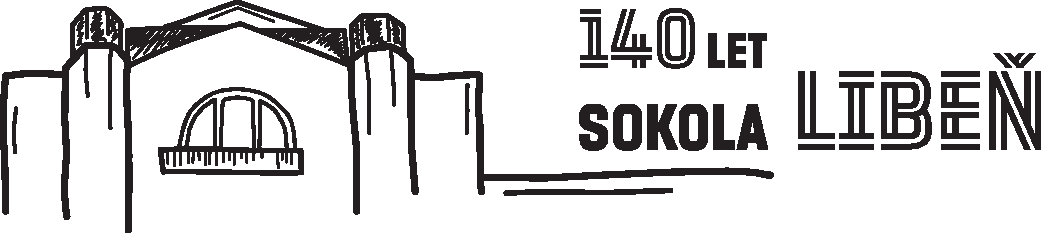
\includegraphics[width=0.7\linewidth]{./logo-140-horiz.pdf}
\end{center}

\subpost{Články do Osmičky}
Vzhledem k~tomu, že Sokol Libeň představuje v~rámci Prahy 8 významnou
kulturně-sportovní instituci, seznamovali jsme v~sérii článků
v~měsíčníku Osmička širší veřejnost s~fungováním jednoty a představili
nejvýznamnější oddíly a pořádané akce.

\subpost{Prapor mužů}
Náčelník jednoty Josef Kubišta (Pepišta) pojal myšlenku, že naší sbírce
praporů něco chybí. Ano, byl to prapor -- prapor mužů, na nějž se
zejména muži složili a ku příležitosti slavnostní tělocvičné akademie a
10. výročí obnovení oddílu mužů jej předali jednotě.

\begin{center}
  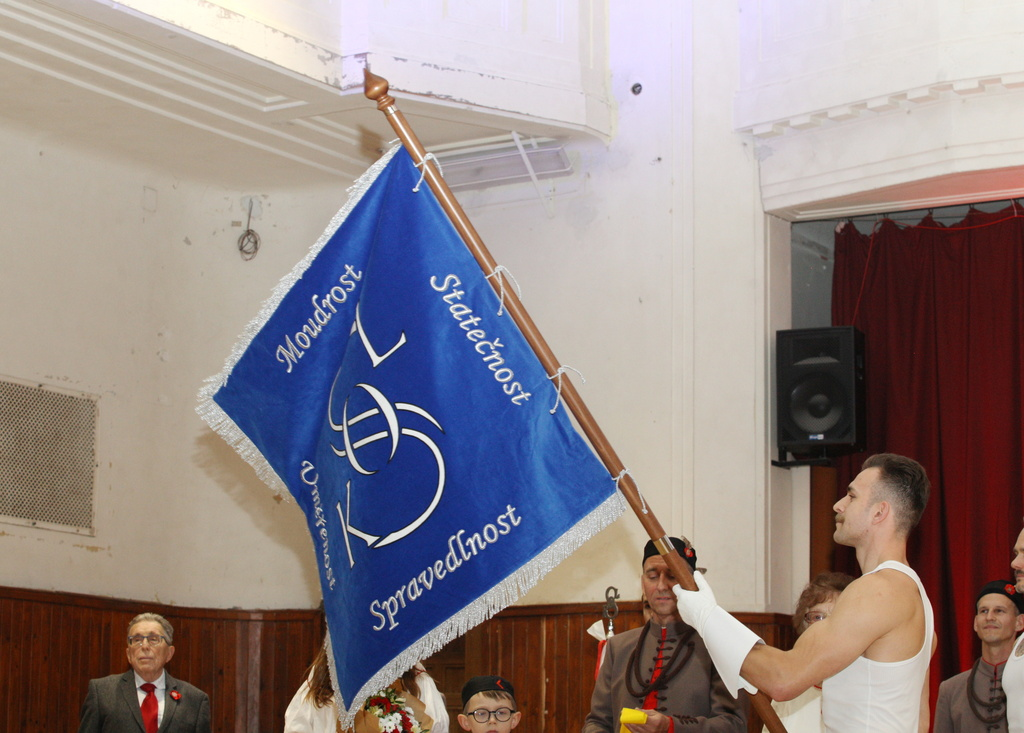
\includegraphics[width=0.8\linewidth]{./FOTKY ZPRAVY/PRAPOR 2.JPG}
\end{center}

\clearpage

\subpost{Fotografie na galerii}
Sokol Libeň je již několik let objektem zájmu fotografa Honzy
Jirkovského. S~jeho pomocí bylo vybráno 16 černobílých fotografií
s~tělocvičnou tématikou, které nyní zdobí galerii naší sokolovny.
Výstava je doplněna o~medailon autora. Nutno dodat, že všechny
fotografie byly pořízeny přímo v~sokolovně, a pokud jste je ještě
neviděli, doporučujeme tyto umělecké kousky Vaší ctěné pozornosti.

\begin{center}
  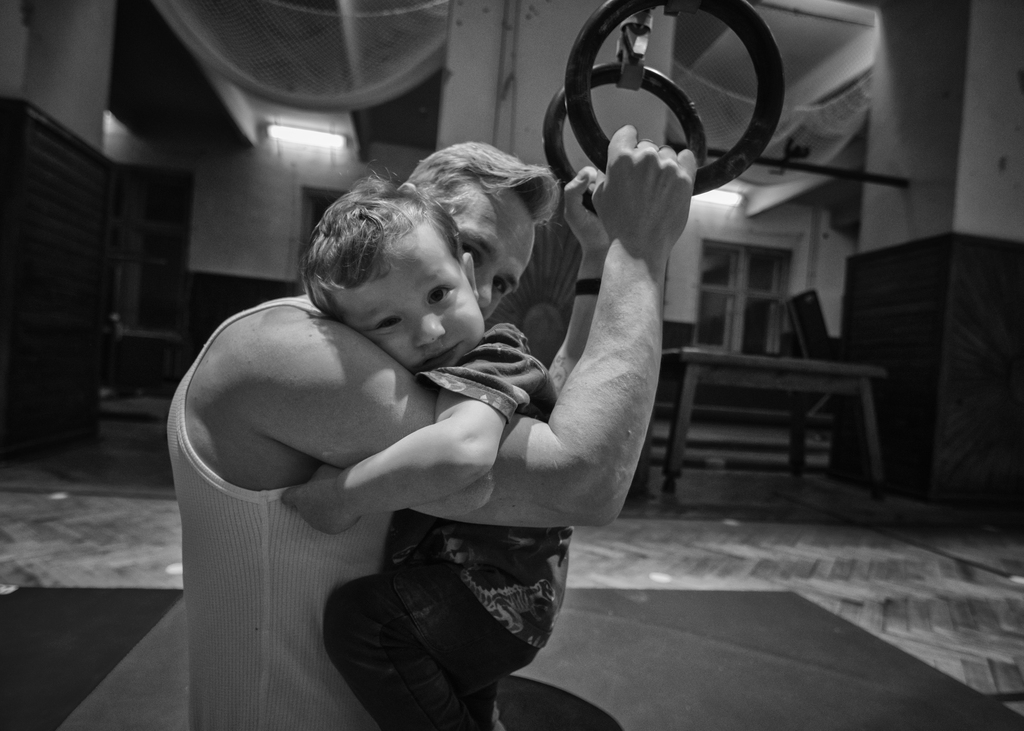
\includegraphics[width=0.7\linewidth]{./FOTKY ZPRAVY/FOTKY GALERIE.jpg}
\end{center}

\subpost{Almanach}
Uvedené výročí nás také přinutilo oprášit a doplnit almanach vydaný ke
120. narozeninám jednoty. Tento nesnadný a časově náročný úkol přijal na
svá bedra jednatel jednoty bratr Jan Přech (Řek), jemuž po grafické
stránce sekundoval Martin Burian, korektorka Martina Waclawičová a další
dobrovolníci.

Křídový papír dodává textu i fotografiím punc důstojnosti, kterou si
vskutku zaslouží. Posuďte sami! Alamanach je vám k~dispozici za
dobrovolný příspěvek 200 Kč ve vrátnici sokolovny. Platba možná hotově
nebo za pomoci QR kódu.

\subpost{Meotarové vystoupení}
Hlavní program oslav, plánovaných na víkend 22.--24. listopadu 2024, byl
zahájen vtipnou exkurzí do historie Sokola Libeň pod názvem "Obrazy
z~dějin Sokola libeňského aneb nevážná meotarová rozpustilost ve věci
dějepravy". Slovem nás provázel začínající "scénárista" Tomáš Troup,
kresby na meotar pokládal jejich autor, občasný karikaturista Jáchym
Kaplan (Jack). Nutno zdůraznit, že neotřelý koncept s~využitím meotaru
sklidil u~diváků nebývalý ohlas. Bylo tedy dle programu rozhodnuto, že
po tak úspěšné premiéře je nutné představení opakovat. A~tak se skutečně
konala tentýž den i derniéra uvedeného kusu. Pokud se posouváním po
meotaru obrázky příliš "neotřely", možná dostanou příležitost i ti,
kteří svou první a "poslední" šanci v~pátek 22. listopadu 2024
propásli.

Z~řad obecenstva dokonce zaznívaly tak troufalé návrhy, že by se
představení mělo postoupit široké veřejnosti například v~nedaleké
knihovně u~Löwita. Tvůrci však mají obavu, aby je nesemlela tamní
nesokolská kritika.

\begin{center}
  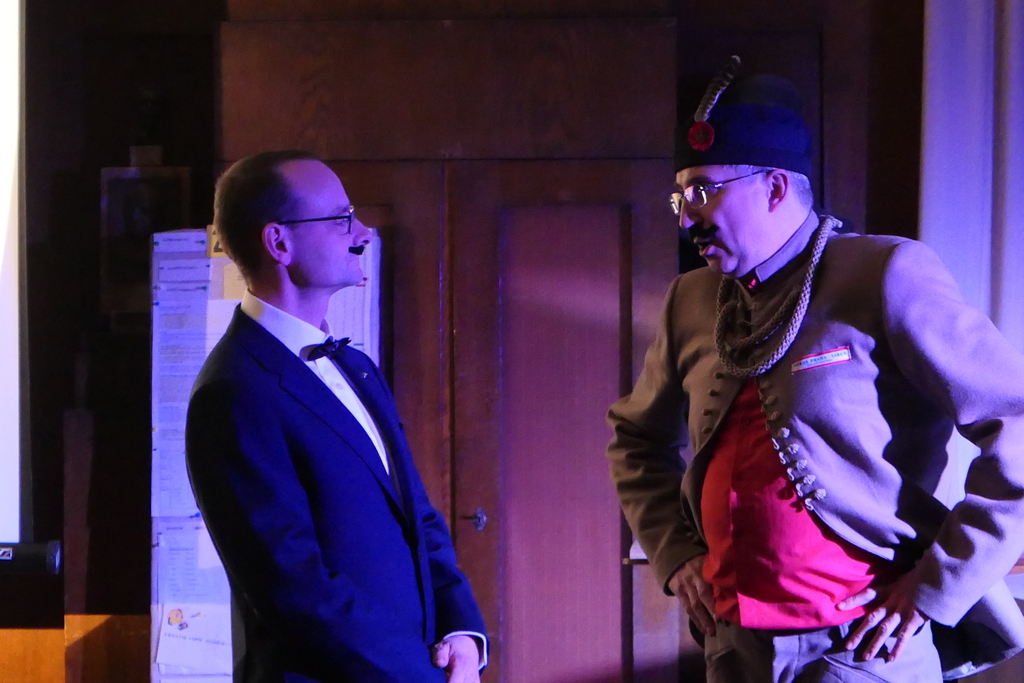
\includegraphics[width=0.7\linewidth]{./FOTKY ZPRAVY/MEOTAR 1.JPG}
\end{center}

\subpost{Výstava}
Po prvním meotarovém vystoupení se valná většina přítomných přesunula do
Alšova sálu na vernisáž výstavy. I~když sálu vévodí skica, jejímž
autorem je slavný malíř Mikoláš Aleš, hlavním předmětem zájmu byla
tentokrát výstava, která pod nepřekvapivým názvem "140 let Sokola
Libeň" umožnila návštěvníkům nahlédnout pod pokličku naší historie a
prohlédnout si alespoň zlomek hodnotných artefaktů, které se k~naší a
sokolské historii pojí. Výstavu připravila dlouholetá vzdělavatelka
jednoty Anna Holanová (Anka), která v~archivu bedlivě střeží všechny
naše duchovní poklady.

V~průběhu víkendového trvání výstavy bylo zajímavé sledovat, jak se
mnozí z~návštěvníků poznávali na dobových fotografiích z~90. let i na
těch aktuálnějších; jak starší vyprávěli mladším, co všechno zažili;
s~úctou procházeli kolem praporů a nejstarších předmětů; připomínali si
bývalé činovníky jednoty a poznávali na fotografiích ty současné;
vzpomínali na jednotlivé všesokolské slety\ldots{} V~neděli po poledni
jsme však naše "rodinné album" zase uschovali do archivu, kde počká i
s~ostatními předměty na další vhodnou příležitost.


\begin{center}
  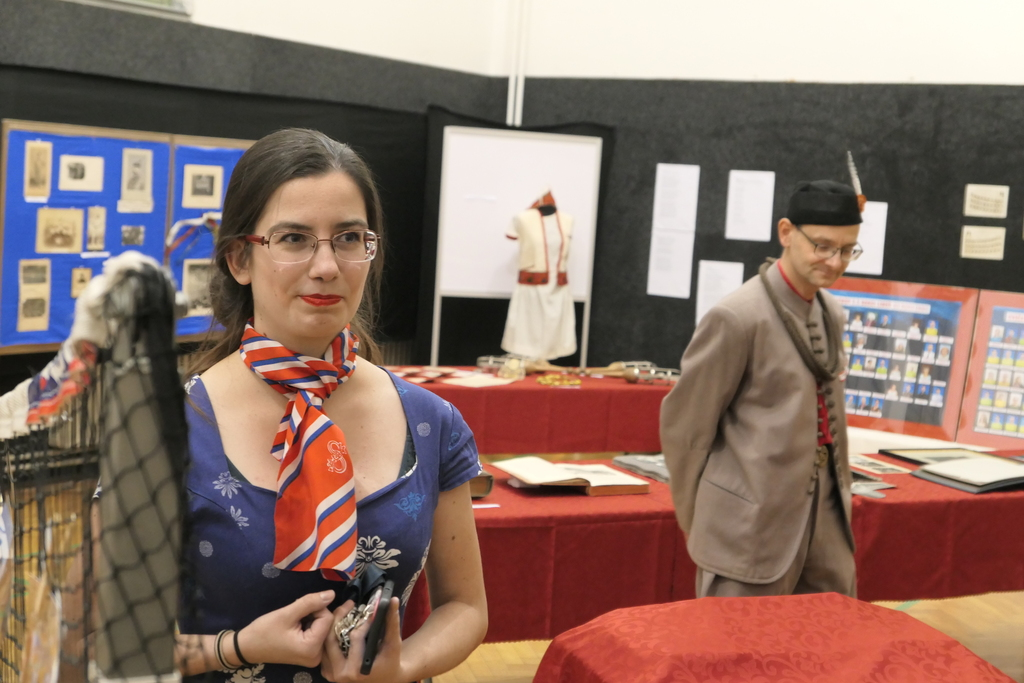
\includegraphics[width=0.7\linewidth]{./FOTKY ZPRAVY/VYSTAVA.JPG}
\end{center}

\subpost{Tělocvičná akademie}

O~této události se zcela jistě dočtete i na jiných místech Zpráv. Abych
však sledoval nit událostí, dovolím si o~ní pojednat v~tomto textu.

Slavnostní tělocvičná akademie se pod taktovkou náčelníka Josefa Kubišty
(Pepišty) konala v~sobotu 23. listopadu 2024 od 16 h. Svou návštěvou
sokolovnu k~této příležitosti poctilo i mnoho významných hostů včetně
starosty městské části Praha 8 p. Ondřeje Grose a starosty České obce
sokolské br. Martina Chlumského.

Při slavnostním nástupu byla sbírka jednotových praporů doplněna
o~prapor mužských složek, který tímto muži věnovali jednotě. Prapor za
doprovodu Foerstrova komorního pěveckého sdružení pokřtila emeritní
členka Sokola Libeň sestra Marie Kselíková. Slavnostní atmosféra byla
dokreslena i zdařilým barevným osvětlením.

O~výbornou atmosféru se po dobu celé akademie starali cvičenci, kteří
předvedli mnoho všestrannostně zaměřených výstupů, i přihlížející
diváci. Cvičební program doplnil i "remake" veleúspěšné scénky "Cvičení
na koni". Nostalgicky jsme také zavzpomínali na mnohé sletové skladby
-- vždyť v~Libni se nacvičovaly téměř všechny\ldots{} Sami diváci svým
potleskem a nadšením dokázali, že se i přes bohatý program čítající
celkem 21 čísel skvěle bavili.

\begin{center}
  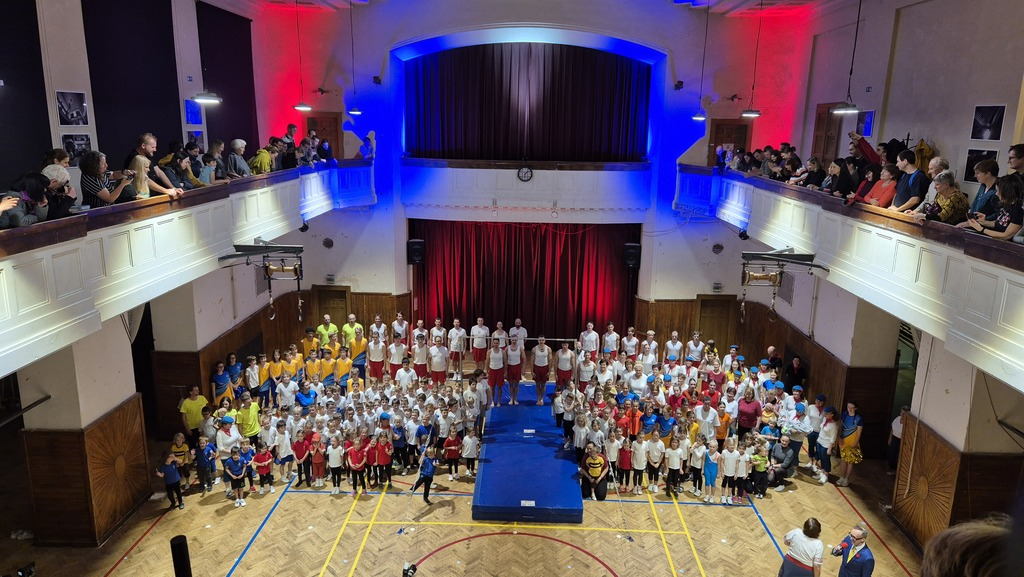
\includegraphics[width=0.7\linewidth]{./FOTKY ZPRAVY/AKADEMIE.jpg}
\end{center}

\subpost{Loutkové divadlo}
Sokol Libeň provozuje již několik let i vlastní ochotnické loutkové
divadlo. Když byl principál Tomáš Troup požádán, zda by soubor v~rámci
oslav nesehrál v~neděli dopoledne pro děti loutkové představení, ochotně
souhlasil a sáhl po (již několikrát) osvědčeném kusu "Tři zlaté vlasy
děda Vševěda". Nevěřící Tomáš byl však od počátku na pochybách, kolik
se tak asi může v~neděli dopoledne sejít diváků\ldots{} Principálovy
pochyby rozptýlily před desátou hodinou až zástupy dětí, které plny
očekávání vlekly své rodiče na zmíněné loutkové představení.

Jistě víte, že zejména mužské složky hoví přesným statistikám. Proto Vám
můžeme přesně sdělit, že diváků, včetně těch dospělých, se nakonec sešlo
nepočítaně, což je opravdu mnoho\ldots{}

Skromným odhadem shlédlo představení asi 80 diváků, kteří zaplnili téměř
celý Srncův sál, jenž sloužil pro potřeby loutkového divadla již ve 20.
letech 20. století.

Dopoledne patřilo dětským divákům, zatímco ti dospělí, jak jste možná
z~několika narážek odhadli, teprve čekali na zlatý hřeb večera.

\subpost{České nebe v~divadle Járy Cimrmana}
Vrcholem oslav 140. výročí byla totiž nedělní návštěva představení České
nebe v~prostorách Žižkovského divadla Járy Cimrmana. Pozitivní,
slavnostní a téměř rodinná atmosféra opanovala divadlo již před začátkem
představení. Úderem 19. hodiny se v~sále setmělo a v~zákulisí začali
nervózně přešlapovat řečníci.

Krátké úvodní slovo pronesl zasloužilý starosta jednoty Jiří Novák
(Jirkan), který krom jiného zmínil i důležitost duchovního rozměru
Sokola. Po starostovi, který dříve přiznal, že v~Sokole Libeň kroutí již
svou 51. sezónu, se na jeviště dostavil náčelník J. Kubišta. Bratr
náčelník však svůj proslov pojal zcela netradičně! Stěžejním prvkem jeho
statě byla analýza stavebního deníku naší sokolovny. Fundovaným a
precizně argumentovaným rozborem překvapil šokované publikum tím, že jej
přivítal, a zde budu raději citovat: "na prknech Sokola Libeň, v~Divadle
Járy Cimrmana!" (Písemný záznam celého projevu máme k~dispozici a
budiž zachován pro věčnou památku této jedinečné návštěvy.)

Náčelníkovi se tak jeho fenomenální cimrmanovsky laděnou přednáškou
podařilo "zbořit" diváky ještě dřív, než přišel sám "Cimrman"!

Náčelníka na jevišti vystřídaly cvičitelky oddílu akrojógy, které na
našich "libeňských" prknech a za zvučného potlesku diváků předvedly své
nevšední akrojogínské umění.

Pak už patřila ta věhlasná prkna jen hercům. Jako první se na jevišti za
bouřlivého potlesku objevil Pan Zdeněk Svěrák (88 let), jenž přítomné
ujistil, že doposud "nevěděl, že hraje na prknech Sokola Libeň"\ldots{}
Jeho účinkování jakožto ikonické, nejen cimrmanovské osobnosti si
nesmírně vážíme; o~to víc, že v~předvečer našeho představení se účastnil
charitativního večera StarDance pro Centrum Paraple! Skvělé bylo celé
představení, takže všech 238 libeňských diváků včetně čestných hostů
(Cimrman by je označil za místní honoraci) v~čele se starostou ČOS br.
M. Chlumským se celý večer výborně bavilo.

\begin{center}
  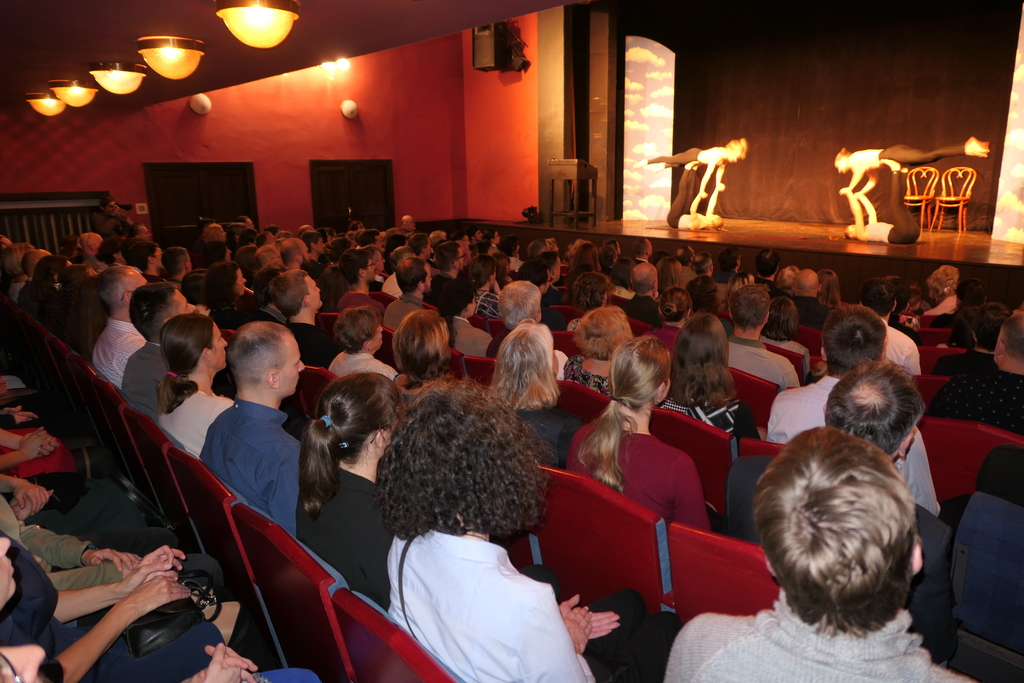
\includegraphics[width=0.7\linewidth]{./FOTKY ZPRAVY/DIVADLO 3.JPG}
\end{center}

Sokol Libeň následně herce obdaroval symbolicky sokolskou kokardou a
výtiskem pamětního almanachu s~věnováním.

Zmíněné představení bylo pomyslnou "pěknou tečkou za tou naší" oslavou.
Pro znavené organizátory se tak stal tento večer motivací k~případným
dalším budoucím počinům podobného ražení.

Závěrem nezbývá než Sokolu Libeň do dalších mnoha let popřát spoustu
obětavých cvičitelů, nadšených dobrovolníků a odhodlaných následovníků,
abychom dokázali i v~dalších letech držet náš sokolský "směr a cíl"!

\vspace*{24pt}

\signature{Miloslav Doupal}{mila.doupal@sokol-liben.cz}

\clearpage

\post{Informace od starosty}

Od posledních Zpráv jsme opět kousek pokročili v~údržbě sokolovny. Co zůstává stabilní, to je počet členů, který je stále okolo 800.

Finanční situace se nám již stabilizovala. Od 1. 1. 2025 nás však opět čeká zvýšení minimální mzdy našich zaměstnanců. Z~18~900\,Kč na 20~800\,Kč za měsíc, tedy o~1~900\,Kč (t. j. o~10\,\%, což v~ročním souhrnu znamená cca 200~000\,Kč).

\subpost{Co nového na dvoře}
Na podzim jsme do nové garáže vyrobili a namontovali držáky na lodě, a mohli tak i zbylé kánoe přesunout do nové místnosti. Stará garáž již byla na podzimní brigádě odstraněna a za sokolovnou tak vzniklo místo pro zamýšlený odpočinkový kout s~ohništěm a kruhem na vrh koulí. Podél zdi budou mít svůj proužek země tahači lanem, kteří si momentálně budují tréninkovou tahací věž se závažím.

V~brzké době budeme muset opravit nízkou zídku z~kyklopského zdiva pod plotem hřiště gymnázia, kde vypadává spárovací omítka i celé kameny.

Pohnula se i situace ohledně kolaudace podzemní místnosti. Po konzultaci se stavebním úřadem už známe postup. Provedou se práce požadované památkáři (odstranění zábradlí, snesení betonového obkladu, zhotovení omítek dle požadavku). Následně si vyžádáme stanovisko památkářů ke kolaudaci a následně o~ni zažádáme na stavebním úřadu. 
V~tuto chvíli již máme volné finance na předělání a stavebně se nejspíše bude řešit na jaře a v~létě roku 2025. 

\subpost{Šatny}
Již jsou ve výrobě držáky na lavice do prostoru vedle schůdku do sociálek a během prosince dojde k~jejich namontování a osazení fošnami na sezení v~provedení jako u~šatnových skříněk a s~deskou s~háčky jako v~šatnových klecích.

K~šatnám ještě jedna prosba k~botníkům. Pokud si nechci boty zamykat, použiju poličku, pokud ano, použiju malý zamykací šuplík a zamknu ho. Větší šuplíky jsou určené pro dětské oddíly, kam se vejde více párů bot. Tak nám je neobsazujte vaším jedním párem – děkujeme. Prázdné šuplíky nechávejte odemčené a klíčky vracejte na háček. Mimochodem, nemá někdo doma klíček od botníku s~číslem 41? Ten už nám nějaký čas chybí.

Hlavním přínosem čistého provozu v~šatnách by měla být i větší čistota v~sálech. Zásada, na které budeme stále striktně trvat, je, že žádné venkovní boty nepřekročí práh šaten (a to ani v~ruce)!!!

\subpost{Další stavební plány}
Firma Wandel nám již udělala projekt na propojení staré matriky s~nájemcem ABA Strategie a v~půlce června podala žádost o~stavební povolení. Před pár dny jsme konečně obdrželi stavební povolení, a 2. prosince by tak měly začít stavební práce, které by však nijak neměly ovlivnit provoz v~šatnách či vlastní cvičení. Hotovo by mělo být do konce roku a od ledna zase budeme moci tyto prostory pronajímat.
V~rámci přítomnosti firmy Wandel, která nám rekonstruovala šatny, budou nahrazeny vadné zámečky skříněk a botníků, bude opraven občas protékající záchod žen v~šatnách a poprosíme je o~výmalbu stropu za dámskými šatnami po jarním protečení vody z~klubovny turistických oddílů.
Do roku 2031 bychom také potřebovali dokončit rekonstrukci dvora (předláždění, nová vrata a vrátka, nový plot), protože nám bude končit platnost stavebního povolení.

A~co pak? Pak se vrhneme na vnitřek sokolovny. 


Jako každý rok se už od jara pilně starám o~nechtěnou (plevel) i žádanou (trávník) zeleň kolem celé sokolovny a snad je to trochu vidět.

Od nového roku jde do důchodu pan vrátný Hofman, jeho směnu převezme paní vrátná Míková.

Do konce listopadu také otevřeme zimní vchod a na ty ostatní opět dáme závěsy, abychom šetřili drahocenné teplo. Také se poprvé spustí podlahové topení v~šatnách. Při této příležitosti prosím všechny cvičence i návštěvníky sokolovny, aby nemanipulovali s~termostaty na radiátorech, a pokud se někde otevře okno, aby se opět zavřelo, a to na obě kličky – děkuji.

\signature{Jiří Novák (Jirkan)}{starosta\\tel.: 602 284 198}


\post{Zpráva místonáčelníka}

\subpost{Cvičení oddílu žáků a dorostenců}
Cvičení venku (park, zahrada sokolovny) s~atletickými disciplínami začalo po prázdninách v~úterý 3. září a skončilo 3. 10. 2024. Od 8. října cvičíme už jen v~sokolovně – kromě gymnastiky nezapomínáme na rozcvičku a hry a brzy jsme zařadili i nácvik na slavnostní akademii ke 140. výročí založení jednoty.

Pevně věříme, že kluci i díky Vám přivedou nové kamarády – rádi uvítáme další zájemce o~cvičení (bereme mladší i starší žáky). Děkujeme a těšíme se. V~loňském cvičebním roce jsme měli zapsáno 136 cvičenců (67 mladších žáků, 39 starších žáků, 13 dorostenců a 17 cvičitelů) a průměrná docházka na hodinu byla 59,835 při měsíčním průměru zapsaných 106,9. Letos je zatím zapsáno 120 cvičenců (51 mladších žáků, 46 starších žáků, 13 dorostenců a 10 cvičitelů) a průměrná docházka na hodinu byla v~září 64,5 a v~říjnu 62,56, ještě o~chlup lepší než loni. A~to loňský rok znamenal pěkný skok nahoru.

Mladší žáci (2015–2018) cvičí v~úterý a čtvrtek od 17 do 18 h, st. žáci a dorostenci (2007–2014) v~úterý a čtvrtek od 18 do 19 h. Pro cvičitele a dorostence je možnost úterního cvičení mužů a čtvrteční košíkové (oboje 19–20 h). 

V~tuto chvíli je už pro žáky spuštěna Zimní soutěž – Hod, kop, střela (počet bezchybných zásahů do malé florbalové branky z~cca 7 metrů při hodu míčkem, kopem a střelbě florbalovou hokejkou). 

Začínáme počítat výsledky letních disciplín (vyhlášení proběhne začátkem roku 2025). Trvá také celoroční soutěž O~nejvěrnější docházku s~pravidelným každoměsíčním vyhlašováním a rozdáváním diplomků za 100\,\% docházku. 

Děkujeme za vzorné zaplacení příspěvků na druhé pololetí roku 2024.

Líbí se vám cvičení mužů na akademiích? Klidně se můžete stát členem oddílu – berou další zájemce (muže 18–50). Cvičí se v~úterý 19–20. 

Výborně funguje před několika lety založený oddíl šplhu (osmimetrové lano ze sedu bez přírazu). Řada jeho členů se účastní i mistrovství republiky v~tomto sportu. Též berou další zájemce od staršího žactva až po muže a šplhají i děvčata a ženy. Další větví v~mnohotvárné činnosti mužů je Přetah lanem – i v~tomto sportu se závodí a konají se i mezinárodní soutěže. Pro lepší trénink jejich oddílu se za sokolovnou momentálně buduje přetahovací věž. 

\subpost{Turistické oddíly}
Všem žákům nabízíme možnost účasti na výletech, které pořádají naše turistické oddíly. Káňata zvou mladší žáky, Jilmáci žáky starší. Mladší děvčata mohou chodit do Káňat, starší do Veverek. Všechny oddíly též samozřejmě nabízejí i členství – což znamená středeční (JILM + Veverky) či čtvrteční (Káňata) schůzky v~klubovně a výpravy, které se konají cca 1x měsíčně. Vyvrcholením celoroční činnosti je pak letní tábor. V~roce 2025 to bude nové místo nedaleko Trhových Svin na Keblanském potoce mezi vesnicemi Něchov a Keblany. Informace u~vedoucích oddílů – viz informace u~oddílů na našich stránkách. 

\subpost{Organizační informace}
Děkujeme za používání matričního systému EOS. Platby příspěvků se nám tak letošní podzim sešly během několika málo dní. Na druhou stranu vás tímto kanálem dokážeme rychle a v~případě potřeby i cíleně informovat o~našich akcích. A~navíc, pokud vy potřebujete něco změnit, máte tak šanci to učinit sami (změna kontaktních údajů, zdravotního stavu apod.), případně lze změnit i oddíl či četnost hodin, a to tak, že se přihlásíte do systému, dáte "Nový požadavek na management" a napíšete, co potřebujete. Kancelář to učiní a dá vám vědět, že se tak stalo. 

V~matrice – 1. patro sokolovny (čtvrtek 15:45–18:45) lze opět za dobrovolný příspěvek obstarat bílé tričko se znakem pro žáky.

O~kluky se stará náš mužský cvičitelský sbor v~tomto složení:
Cvičitelé: J. Novák (53), T. Novák (51), J. Kudroň (35), J. Přibyl (32), J. Kubišta (31), J. Kerhart (21), P. Boháč (20) a naši mladí pomahatelé: J. Skokan, T. Kléger, V. Novák, V. Blahunek, J. Pikálek a A. Basseville. 

Výsledky závodů, fota, dopisy a další informace najdete na vývěskách v~sokolovně a na ní a také na www.sokol-liben.cz. Informace o~důležitých akcích pak putují i přes přihlašovací systém EOS.

Na akademii byl představen nový vzhled i uspořádání našeho webu. V~tuto chvíli se do něj nahrávají a upravují data. Ne vše je ještě doladěno. Po Novém roce už by měly být naše nové stránky plně funkční. Dělali ho naši mladí cvičitelé, tak jim prosím odpusťme počáteční neduhy. 



\subpost{Pronájem sokolovny}
V~pátek a sobotu 13.–14. září se v~sokolovně konala oslava 100 let firmy Emil Frey. Firma si pronajala sokolovnu a zařídila občerstvení, naši cvičitelé jim udělali sportovní a cvičební program na míru dle přání. Nechyběly ani masáže a fyzioterapie, loutkové divadlo, vystoupení Skipping Buddies, sletového Sokolhraní, akrojógy a mužů na nářadí. Pomáhalo 41 cvičitelů a pomocníků a bylo k~tomu ještě 24 vystupujících. Vydělali jsme si pěkných 300~000\,Kč.

\subpost{Běh strmý}
Ve čtvrtek 19. září se konal 24. ročník Běhu strmého do zámeckého vrchu. Běželo se 199 metrů s~převýšením 29 metrů v~libeňském parku. V~nepříliš příznivém počasí (mžení, 18\,°C) dorazilo solidních 179 závodníků ve všech vypsaných kategoriích. Největším počtem závodníků se mohla pochlubit kategorie mladších žáků – bylo jich 39. Krátce po doběhu posledního závodníka začalo vyhlašování vítězů. První tři v~každé kategorii si odnesli diplom, sladkost a drobnou věcnou cenu. Vítěz pak ještě plastiku sokolíka (nově z~3D tisku). Absolutním vítězem se stal časem 38,7 V. Paleta. Padl rekord kategorie seniorů – J. Prahl, 42,5. Všichni běžci si odnesli pamětní lísteček a drobnou sladkost. Došlo i na tradiční foto vítězů s~putovním pohárem. Děkujeme všem 18 pořadatelům.

Cvičitelé (23 osob) se po Běhu strmém sešli na pracovní schůzce ve sborovně, kde si rozdělili pořadatelství akcí a další úkoly, a také jsme určili data všech akcí až do června 2025.

\clearpage
\subpost{Noc sokoloven}
V~pátek 27. září se v~sokolovně konala Noc sokoloven. Jejím letošním mottem byl šplh, na počest 1. české zlaté olympijské medaile Bedřicha Šupčíka v~Paříži 1924. Akce tedy začínala v~17 hodin, kdy mají trénink naši šplhači. Každý z~příchozích si mohl zkusit vyšplhat. Další zájemci si v~druhé části sálu mohli zahrát fotbálek a florbal. V~lodi byla k~dispozici trampolínka a bedna na přeskok. Posledním bodem programu bylo promítání na strop sokolovny. Poměrem 18:2 vyhrálo Sokol gala nad 2. programem sletu. Prý to bylo krásné. Ležet na žíněnkách a nad hlavou sledovat ta hezká vystoupení. Celkem bylo 48 osob – 18 šplhačů a 30 návštěvníků.

\subpost{Památný den sokolstva}
Na Památný den sokolstva v~úterý 8. října byla pro zájemce připravena dobrodružná cesta kánoemi z~Libně do Tyršova domu. Zájemci z~řad sokolů z~celé Prahy mohli do Tyršova domu a následně k~Čertovce na pouštění sokolských světel dorazit buď pěšky, anebo na kolech v~rámci spanilé jízdy. Župní vzdělavatel a Zdeněk Lauschmann nás požádali o~třetí dopravní prostředek, tedy lodě. Našli se čtyři dospělí (J. Kudroň, A. Holanová, O. Růžek a S. Vinkler) a k~nim se přihlásily 4 děti (P. Ettel, K. Bílek, L. Bednář a A. Vinklerová). 
Vyrazili v~16:45 po Rokytce, po slepém rameni Vltavy a pak proti proudu Vltavy pod libeňský most, do zdymadla na Štvanici a dále proti proudu Vltavy až do Čertovky, kde chtěli být v~18:15, aby stihli ono pouštění lodiček v~18:30. Jenže z~přehrad nad Prahou se ještě upouštěla vody po nedávných povodních a protiproud byl nečekaně silný. Už po zdymadle museli nasadit čelovky a do Čertovky připluli až v~19:30. Na místě se pozdravili s~ještě přítomným starostou ČOS Martinem Chlumským, naložili lodě na vozík a vrátili se do Libně MHD. Ale zážitek z~té akce prý mají všichni pěkný, i když vlastní akci nestihli. 

Ve čtvrtek 10. října proběhl pietní akt k~Památnému dni sokolstva v~sokolovně. Nejprve proběhlo položení květin u~pamětní desky obětí II. světové války na chodbě před Strnadovým sálem (jednotový prapor, 12 krojovaných sokolů) a následoval proslov náčelník Josefa Kubišty. Pak se většina ze 130 přítomných přesunula nejprve k~soše Jana Podlipného (položení květiny) a následně k~Rokytce, kde každý vypustil lodičku se svíčkou na památku sokolských obětí německé okupace.



\subpost{Podzimní Výlet Libeňského Sokola}
Podzimní Výlet Libeňského Sokola (již 67. v~pořadí) byl v~sobotu 12. října. Opět jsme se připojili ke Srazu v~přírodě pražských žup. Ono to je tedy spíše naopak, protože ze 117 přítomných bylo 83 z~Libně (37 z~našich turistických oddílů JILM, Veverky a Káňata a 46 dalších cvičenců, rodičů a hostů). Ze srazu na Palmovce se jelo metrem na Hlavní nádraží a pak vlakem do Dobřichovic. Kousek od nádraží jsme si zahráli hříčku s~chytáním všech ostatních hráčů na čas. Pak už dalším vlakem dorazili ostatní účastníci i pořadatelé ze Sokola Zlíchov a společně jsme se vydali asi kilometr proti proudu Berounky na zahajovací nástup. Zazpívali jsme si písničku, vyhlásila se Pamatovačka, Jazykohrátky a Vaření a už se šli zájemci smočit v~trošku rozvodněné Berounce, která měla teplotu 12,5 °C a obdrželi tak Modrou stuhu (bylo to pouze 23 lidí). 

Následoval přesun se stoupáním k~vrcholu Červená Hlína. Asi v~polovině trasy byla přestávka na svačinu a hříčku Na ocasaté – šestice hráčů držící se v~zástupu se snaží prvním členem družstva vytrhnout ocas (šátek) poslednímu členovi jakéhokoli dalšího družstva. Po hře jsme dokončili stoupání na vrchol a vystoupali i na jen asi dva roky starou rozhlednu Korunka, ze které byl nádherný výhled na Brdy, blízké Černolické skály, Radotín, vysílač Cukrák i Prahu. Následoval oběd na ohni a Vaření soutěžní polévky. Pak ještě proběhla hříčka Veverky – sedmice se drží za ruce a alespoň jeden krajní člen se musí vždy dotýkat kmene stromu. Úkolem byl co nejrychlejší přesun lesem do asi 200 m vzdáleného cíle.

Pak už byl zakončovací nástup s~vyhlášením jednotlivých soutěží a rozdáním Pamětních lístečků. A~individuální přesun skupinek na vlak a cesta zpět do Prahy. Jarní výlet proběhne 12. dubna 2025.

\subpost{Závody a hra na Starém Městě}
V~pátek 8. 11. proběhla tradiční plavecká štafeta O~pohár starostů pražských žup. Naše župa obsadila v~dětské kategorii 1. místo (z~Libně A. Musil, O. Nekvapil, V. Neumanová, J. Dudová a K. Vránová) a v~dospělé kategorii 2. místo mezi třemi pražskými župami. Za Libeň závodili L. Šimek a T. Lašek. 

V~sobotu 9. 11. měli Jilmáci a Veverky již 44. ročník hry Vyzvědači. Tři skupiny navzájem zjišťují na území protivníka potřebné věci a sami tomu na svém území brání. Hrálo 14 dětí a 6 vedoucích.

\subpost{Brigáda}
V~sobotu 9. 11. byla také Podzimní brigáda. K~práci se sešlo 29 lidí pracantů (10 cvičitelů, 2 cvičitelky, 2 žáci, 1 žákyně, 2 ženy a 12 mužů), kteří se po rozdělení prací postarali o~následující činnosti: v~sokolovně se vysál prach nad pamětní deskou a na římsách zábradlí galerie a balustrády, zatloukly se povylezlé hřebíčky obložení sálu, připravilo zavěšení pro fotografie na galerii, přestěhovaly se skříně a koberce z~galerie a chodby, odstranily dočasné modré sletové značky, opravilo zavěšení poličky v~nářaďovně, odnosily se věci z~dílny na půdu, prohodily se dva stroje v~posilovně, upravily se výřezy v~žíněnkách pro bradla a uklidila se nářaďovna Srncova sálu. 
Venku jsem již v~pátek prořezal tis na tarasu a šeříky před kostelem a dnes došlo na zpracování větví. Vyklidila se garáž a věci z~ní se uklidily, případně se s~rozloženými zbylými šatnovými skříňkami odvezly do sběrného dvora. Dále se pohrabalo listí před kostelem a zametlo se před sokolovnou a chodník nad doskočištěm. Byla sešita roztržená krycí plachta doskočiště, ve fasádě byla maltou začištěna díra po komínku plynového kotle. Nejrozsáhlejší prací však bylo rozebrání staré plechové garáže za sokolovnou. Plechy i jekly se uklidily do dílny pro plánované použití turistickými oddíly na stavbu boudy pro podsady a další vybavení na novém tábořišti. Dokonce došlo i na rozbití betonu pod garáží. Po jeho odvozu (asi 10 m3) se nechá dovézt náklaďák hlíny a místo se na jaře zatravní.
Pracovali jsme od 9 ráno do 5 odpoledne (to už byla tma) a odpracovali 173 hodin.

V~neděli 10. 11. byla brigáda turistických oddílů. Sešlo se 12 dětí a 5 vedoucích a od 9 do půl druhé stihli vykonat následující práce: úklid klubovny a táborového vybavení v~dílně, úklid dílny, převožení kompostu od tahací věže ke kompostérům. Odpracovalo se 76 hodin.

\clearpage
\subpost{Oslavy 140. výročí založení Sokola Libeň}
Cvičitelé a Míla Doupal začali v~září s~intenzivnější prací na 140. výročí založení jednoty. Už od ledna vycházejí v~měsíčníku Osmička městské části Prahy 8 články o~naší jednotě, v~září se v~sokolovně objevila "muší křídla" s~logem oslav, začaly se sepisovat články do připravovaného almanachu. Přemýšleli jsme, jaké vzácné hosty pozvat na naše oslavy. Muži si již na jaře navrhli k~10. výročí obnovení oddílu svůj oddílový prapor, který se právě v~říjnu dokončoval atd. 

V~druhé půlce listopadu se zintenzivnily jak nácviky vystoupení na akademii, tak i další práce související s~oslavami 140. výročí. Dokončily se články pro almanach, vše prošlo korekturou a byl zadán tisk. Vzdělavatelka dokončila sběr fotografií a začala vytvářet tabla – jedno výborové a druhé cvičitelské. Také začala s~pomocí několika pomocníků připravovat výstavu v~Alšově sále. A~nakonec vše vypuklo.

V~pátek 22. listopadu vše začalo. V~18:30 se nás sešlo asi 30 a shlédli jsme více než půlhodinové představení Tomáše Troupa (principála loutkového divadla Nástup) o~vzniku libeňského Sokola nazvané Obrazy z~dějin Sokola libeňského aneb nevážná meotarová rozpustilost ve věci dějepravy. U~meotaru mu pomáhal Jáchym Kaplan a v~živých scénkách Míla Doupal. Opravdu jsme se bavili a po skončení představení zazněla vedle pochvaly i podmínka, že následná derniéra musí být natočena a uchována pro příští generace. Takže i vy ostatní se budete moci časem pobavit na našem YouTube kanálu díky této historické fikci.

Ihned po skončení výše zmíněného představení jsme se přesunuli do Alšova sálu, kde proběhla krátká vernisáž výstavy k~našemu výročí. Na výstavě byly k~vidění naše historické prapory i kroje, fotografie z~různých období, různé historické artefakty – obrazy, členské legitimace, nádobí, cvičební náčiní, štafetové pochodně, básně, jilmácké kroniky a také novinka – tablo členů výboru jednoty od roku 1990 do dnešních dní a dále také tablo s~fotografiemi cvičitelských sborů za posledních 5 let. Krátce po zahájení výstavy došlo také na netradiční křest našeho nového almanachu, který převzal texty a navázal na almanach z~roku 2004. Novému almanachu Nazdar! Zdar!!! Výstava byla otevřena i v~sobotu před akademií a po ní a v~neděli dopoledne.

Večer ještě náčelník s~několika pomocníky nainstaloval na galerii výstavu fotografií libeňských cvičenců od Jana Jirkovského a také byla usazena zapůjčená barevná světla.

V~sobotu 23. listopadu jsme se v~9 hodin sešli na přípravu akademie. Přišlo 51 lidí (15 cvičitelů, 5 cvičitelek, 23 žáků, 6 mužů a 2 ženy). Uklidilo a připravilo se nářadí, vysál se prach, z~kotelny se nanosila pódia, na ně se rozmístilo 217 židlí, připravila se režie a ozvučení, poklidila sokolovna, 2x se před ní zametlo listí, připravily se koridory pro diváky a stolek na schody, roznosili jsme věšáky na kabáty a v~11 hodin bylo vše připraveno a mohly začít naplánované generálky některých vystoupení. Ty trvaly do 15:45. Pak rychle přivést žáky, rozdělit je a usadit na lavičky pro cvičence.

V~16:00 začíná akademie. Židle v~sále jsou obsazeny, dalších asi 150 lidí stojí na galerii. Z~čestných hostů se dostavil starosta Prahy 8 Ondřej Gros a radní Štorek, Blahunková a Musilová, ze župy dorazil starosta Luděk Pokorný a náčelník Petr Čížkovský, z~jiných jednot dorazila Věra Čížkovská, Anička Jurčíčková (bývalá náčelnice ČOS), Marie Hamplová, Lenka Brandová, z~našich zasloužilých členů pak Marie Kselíková a Zdeněk Lauschmann. V~druhé půlce akademie pak z~výboru ČOS dorazil i současný starosta a náš člen Martin Chlumský. Ze zdravotních důvodů se omluvili a akademii pozdravili naši bývalí členové Jiří Sixta a Evža Hraničková. Omluvu poslal i radní magistrátu pan Hanžlík a náčelnice ČOS Eva Řibřidová a náčelník ČOS Petr Svoboda. 

Z~balustrády zapěly Foerstrovky (25 pěvkyň) a už se na plochu šine 40 lidí s~praporem, v~krojích a historických cvičebních úborech. Moderátor Jan Přech vítá hosty, řeční starosta Prahy 8 O. Gros i starosta libeňského Sokola Jiří Novák. Náčelník Josef Kubišta přichází s~novým mužským praporem, který je slavnostně představen a kmotrou praporu Marií Kselíkovou opatřen stuhou. Znovu zpívá Foerstrovo komorní sdružení. Prapory odcházejí a začíná cvičební část. 

Jako první řádilo na ploše se švihadly 4 + 13 členů Skipping Boys a Skipping Buddies, po nich přichází historická Česká Beseda v~podání 16 cvičitelů a cvičitelek v~historických krojích. Kvůli včerejšímu zranění musely svoji účast odvolat Cheerleaders. Místo toho vystoupila komická dvojice Pepišta a Hopi s~"cvičením" na koni našíř. Následovalo cvičení 12 párů Rodičů a dětí nazvané Kakadu. Pod vedením 7 cvičitelů se s~poněkud neobvyklým a netradičním cvičením na kruzích a žíněnkách předvedlo 24 starších žáků a dorostenců. Nápady dodal náčelník Josef Kubišta. Pod vedením Dany Cejpkové zacvičilo 26 předškoláků se 4 dospěláky skladbičku Sandály.

Následoval první sletový blok s~ukázkami skladeb z~letošního sletu: Sokolhraní (16), Čmeláci (24), Jdi za štěstím (20 hostů z~různých jednot), Mravenci (20), Čarodějky (18). Dalšími hosty byly Mažoretky ze Sokola Vysočany (8). Dále zacvičilo 29 mladších žákyň se 4 vedoucími pódiovku Stonožky pod vodou a 34 žáků předvedlo s~8 cvičiteli nápadité cvičení se šplhacími tyčemi, které posloužily jak pro běhavou rozcvičku, tak pro cvičení na hrazdě i pro přeskoky švihadla. Nakonec došlo i na ten šplh. Starší žákyně (24) zatančily s~dřevěnými tyčemi a už je tu druhý sletový blok: Babí léto (8), Před kamerou (18), Fitness (12 + 12), V~rytmu srdce (22). Jako poslední nastoupilo na plochu 20 mužů a předvedlo krásné silové cviky na hrazdě. Pak už jen nástup všech cvičenců a akademie je za námi.

Děkujeme technické četě, režii, "hostesce" u~vstupu, fotografům a samozřejmě i 350 divákům za uznalý potlesk a hlavně všem 330 cvičencům (300 Libeňáků, 30 hostů) a jejich cvičitelům za krásná vystoupení. V~neposlední řadě i rodičům dětských cvičenců, že jim na akademii umožnili nácvik a účast, protože to pro ně byl krásný zážitek a akademie se jim moc líbila. 

Vedení se šlo do Filipovy síně věnovat vzácným hostům, cvičitelé a starší žáci pak během hodiny opět uklidili všechny židle, pódia, nářadí, opět se namontoval basketbalový koš a nikdo nepoznal, že se tu dnes něco dělo. Někteří diváci ještě navštívili výstavu a nakonec se všechno cvičitelstvo sešlo na občerstvení ve Filipově síni, kde jsme akademii zhodnotili, a to velmi kladně.

V~neděli dopoledne pokračovala výstava a bylo představení loutkového divadla Nástup – Tři zlaté vlasy děda Vševěda. Podívat se přišlo asi 70 diváků.

Večer proběhlo zakončení oslav návštěvou skoro 200 Libeňáků v~Žižkovském divadle Járy Cimrmana na představení České nebe. Na začátku večera jsem měl proslov k~divákům a neodpustil si tři cimrmanovské hlášky. Po mě nastoupil náčelník a ten měl proslov v~podstatě o~tom, že Jára Cimrman (stavitel Jarouš), pod jehož vedením šla stavba neuvěřitelně rychle kupředu, se po neshodě se starostou Fr. Filipem rozhodl na stavbě skončit a odvezl nějaká prkna a hřebíky, která se následně dostala do žižkovského divadla. Na konci představení po děkovačce pan Svěrák prohlásil, že do této chvíle netušil, že hraje na prknech libeňského Sokola.

Bylo to vydařené představení. Stejně jako celé oslavy.

\subpost{A~co nás čeká ve cvičení v~nejbližších dnech a měsících?}

Ve čtvrtek 5. prosince Mikuláš spolu s~čerty a anděly zavítá do naší sokolovny a přinese snad i nějaké balíčky pro hodné (a přihlášené) děti.

V~neděli 8. 12. pořádá Sokol Kobylisy soutěž Rychlý šplhoun. Zájemci, hlaste se u~cvičitele Jana Pikálka.

Ve středu 19. 12. bude mít vánoční nadílku oddíl JILM + Veverky a ve čtvrtek 20. 12. pak Káňata. 

Ve čtvrtek 19. 12. sehraje loutkové divadlo libeňského Sokola Nástup od 17 hodin hru Vánoční sokol. Přijďte se podívat.

\textbf{Poslední cvičení v~roce 2024 bude ve čtvrtek 19. 12.}, po Novém roce se sejdeme pro zájemce ještě o~prázdninách ve čtvrtek 2. ledna 2025, oficiálně pak začne cvičení v~úterý 7. ledna 2025.

V~pátek 3. 1. 2025 se cvičitelé sejdou na Silvestru cvičitelů. Kromě zábavy i promyšlení jarních akcí a doladění přípravy nového tábořiště. 

V~úterý a čtvrtek 11. a 13. února proběhnou Nominační závody pro žáky – výběr šikovných žáků na dubnové závody všestrannosti. 

V~sobotu 15. února proběhne další ročník Memoriálu Jana Vorla – gymnastické závody pro muže a dorostence. 

Ve čtvrtek 27. 2. sehrají loutkáři od 17 hodin v~Srncově sále hru Sokolské peklo.

V~neděli 2. března pak bude tradiční jarní brigáda. 

V~sobotu 8. března nás čekají dětské i dospělácké Šibřinky 

Ve středu 19. března proběhne Valná hromada – potřebujeme nejen delegáty na Valnou hromadu za oddíly, ale rádi občerstvíme novými tvářemi i výbor jednoty. Zájemci o~tuto činnost nechť se hlásí starostovi.

Program máme opravdu bohatý, mimo vlastní cvičení dáváme mnoho nabídek na akce s~různým zaměřením. Stačí si jen vybrat a připojit se k~nám. Těšíme se na setkání.

Do dalších let přeji libeňskému Sokolu zapálené a obětavé cvičitele a činovníky, kteří nastavenou laťku alespoň udrží, ale lépe ještě posunou o~kousek výš, cvičence, kteří budou mít chuť se hýbat, a dále dostatek financí na potřebné opravy a vybavení. 

Všem pak přeji klidné předvánoční období i vlastní Vánoce a po Novém roce se těším na další setkávání


\signature{Jiří Novák (Jirkan)}{místonáčelník\\tel.: 602 284 198}

\vspace*{24pt}

\begin{center}
  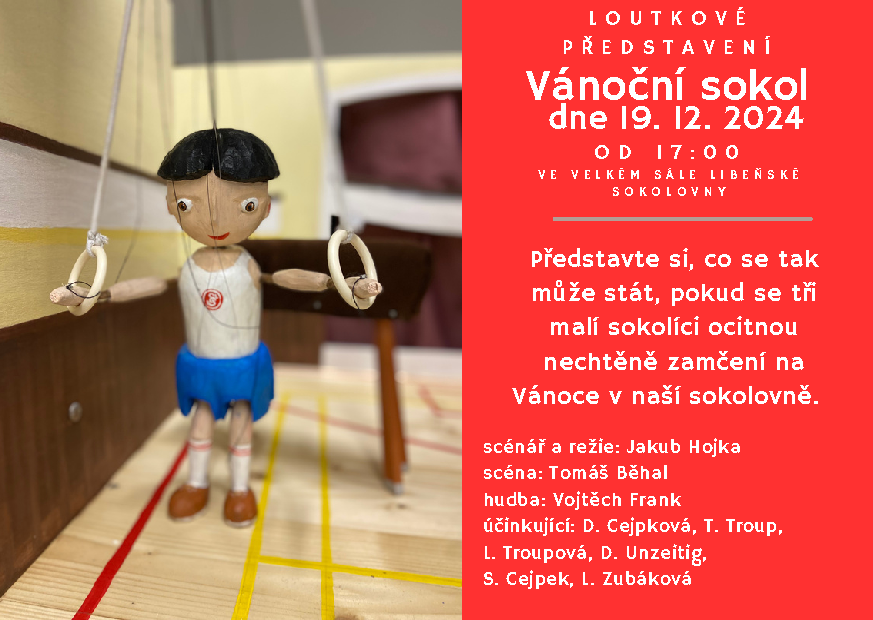
\includegraphics[width=\linewidth]{./Vanocni_Sokol_sal_2024.pdf}
\end{center}

\vspace*{24pt}

\post{JILM a Veverky}
Náš oddíl dále pokračuje. Máme za sebou společný tábor na tajanovské louce se společným programem. První a na dlouhou dobu jediný spojený tábor byl v~roce 2012, kde ale oba oddíly měly rozdílný program a řád. Po 12 letech se tak najednou pod stejným stožárem sešli dívky i chlapci z~řad Veverek i Jilmáků. Zároveň jsme měli naposled postavené stany u~Velhartic, naše vybavení zatím odpočívá ve stodole u~Pešulů. Příští rok bude náš tábor stát na nové louce u~Trhových Svin i s~novými podsadami.

\vspace*{\baselineskip}
\noindent
Co jsme prožili:
\begin{itemize}[
  itemsep=-3pt,
  leftmargin=1em,
  itemindent=-1em
]
  \item[] O~víkendech 21.–⁠⁠⁠⁠⁠⁠23. 6. a 19.–⁠⁠⁠⁠⁠⁠21. 7. jsme společnými silami současných i bývalých členů, vedoucích, rodičů a dalších ochotných lidí postavili kompletní tábor na tajanovské louce.
  \item[] Ve třech týdnech od 10. do 31. 8. si 19 členů a až 9 vedoucích užilo konec prázdnin na táboře. Nechyběl program z~tradic obou oddílů (modrá stuha, červená tuhá/antituk, ruletahni\,\ldots{}). V~rámci celotáborové hry jsme se přesunuli do Kralických hor, kde jsme měli za úkol pochytat pašeráky a vyřešit záhadnou vraždu Bety Krausové.
  \item[] V~sobotu 12. 10. jsme se vypravili na PVLS, který letos připravil Jakub –⁠⁠⁠⁠⁠⁠ Koblížek ze Zlíchova, na rozhlednu Korunku k~Dobřichovicím a v~neděli jsme navázali kolovkou z~Kralup nad Vltavou zpátky k~naší sokolovně.
  \item[] Jedno listopadové odpoledne 9. 11. se sešlo 14 členů na dobrodružnou hru Vyzvědači. Se šťastným nálezem hromady výkupného vyhrála družina modrá s~430 body, za ní žlutá s~398 body a bronz sklidila zelená s~315. Následující den, v~neděli 10. 11., jsme poklidili v~klubovně, dílně a na dvorku.
\end{itemize}

\vspace*{\baselineskip}
\noindent
Co nás čeká:
\begin{itemize}[
  itemsep=-3pt,
  leftmargin=1em,
  itemindent=-1em
]
  \item[] Vánoční výprava –⁠⁠⁠⁠⁠⁠ 13.–⁠⁠⁠⁠⁠⁠15. 12. se vydáme do krásné zimní krajiny.
  \item[] Vánoční nadílka 18. 12.
  \item[] Přespání v~sokolovně a jednodenní výprava 10.–⁠⁠⁠⁠⁠⁠11. 1.
  \item[] Zimní táboření 30. 1. –⁠⁠⁠⁠⁠⁠ 2. 2.
\end{itemize}

\noindent
Jakékoliv dotazy nebo podněty pište na náš e-mail jilmveverky@sokol-liben.cz.

\signature{Bára}{}

\post{Akrojóga}
Od září se toho v~libeňské akrojóze spoustu událo. Konaly se již 3 akrolekce a 4. nás čeká v~prosinci 13. 12. a v~mezičase se oddíl rozrostl o~mnoho zájemců, přičemž v~listopadu dorazil rekordní počet 20 lidí! Zároveň jsme se v~listopadu podílely hned na 2 vystoupeních pro Sokol. První bylo 17. listopadu před Národním divadlem jako úvod k~sokolským přednáškám, druhé hned o~týden později 24. listopadu v~Žižkovském divadle Járy Cimrmana v~rámci oslav výročí 140 let Sokola Libeň.

Akrojóga je cvičení v~páru, které propojuje akrobacii, gymnastiku a jógu. Jeden ze dvojice, tzv. letec, létá vzduchem a cvičí na svém partnerovi, tzv. bázi, která většinou leží na zemi, případně stojí. Oba dva řádně procvičí rovnováhu a koordinaci, zapojí celé tělo,

zaposilují si i se protáhnou. Navíc je cvičení i o~důvěře v~druhého a o~vzájemné komunikaci. V~akrojóze letec cvičí jednotlivé samostatné prvky, které může následně jakkoli propojit a poskládat v~sestavu, tzv. flow. Flow může být krátké a jednoduché, nebo delší a složitější s~různými skoky do vzduchu, otočkami a stojkami.

Již druhým rokem pořádáme v~Sokole 1x měsíčně akrolekce pod naším vedením – akrodvojčat Aničky a Markéty. Nejsme profíci, ale baví nás zkoušet nové a nové cviky a rády předáváme to, co samy umíme, dál. Akrolekce jsou určené pro všechny zájemce jakékoli úrovně, fyzické zdatnosti, věku a pohlaví. Další lekce proběhne v~pátek 13. prosince v~18:00–19:30 v~lodi hlavního sálu v~sokolovně. Pro členy Sokola je lekce zdarma, pro nečleny je cena 100 Kč. S~sebou je potřeba jen sportovní oblečení.

V~případě dotazů můžete kontaktovat Markétu Kolářovou na čísle 736 762 307 či e-mailu marketa.kolarova@sokol-liben.cz.

Na všechny se těší

\signature{Anička a Markéta}{}


\post{Oddíl rodičů a dětí}
\subpost{Míčový trojboj 17. 11.\\není důležité množství hráčů, ale chuť vítězit}
Každý rok se v~Sokole Karlín konají celopražské závody v~Míčovém trojboji, kdy v~kategorii nejmenších dětí nezávodí jen dítě, ale samozřejmě i rodič. Už léta se potýkám s~tím, že malí závodníci by byli, ale ti velcí – rodiče mají problém, zda svému dítěti nepokazí na závodech výsledek.

Nikdy však nepodceňujeme trénink, a tak rodiče trápí ve prospěch svého dítěte sami sebe, aby při střelbě na koš hodili tu trojku, kterou většinou házeli naposledy na gymplu. :-) Myslím, že je super, že i děti vidí, že rodičům něco nejde a že i jim to dá pěkně zabrat, aby něco zvládli. Především to však zkouší a nevzdávají a to je ten důležitý vzor, který by si mladší dítě mělo od svých rodičů přebrat. 

\begin{center}
  \includegraphics*[width=0.7\linewidth]{./RD_zavody.jpg}
\end{center}

Často nemoc nejmenších závodníků krutě zasáhne do předem zaslané soupisky. Letos tomu nebylo jinak, kdy z~8 nahlášených párů se jich zúčastnily 4. Mezi jednotlivými sokolskými jednotami panují velmi přátelské vztahy, tak se libeňští kluci spojili s~kluky z~Vršovic a holčičky se přiřadily k~družstvu ze Sokola Prahy VII.

V~obou týmech byly libeňské děti velkým posilami, protože 2 děti měly individuální medaile: 2x stříbrnou. Po hodně dlouhé době se stalo, že i v~kategorii párů, kdy body sbírá nejen dítě, ale i rodič, vyhrál pár z~Libně. Bylo to rozhodně dáno chutí obou závodníků užít si to a dát do toho vše.

Děti si ještě v~kategoriích družstev odnesly stříbrné (kluci) a zlaté (holky) medaile.

\subpost{Mikuláš a loutkové představení}
Dne 5. 12. přišly do hodiny rodičů a dětí nebeské bytosti. Děti si opět odnesly plné látkové balíčky, které, když zkonzumují jejich obsah, mohou používat po celý rok např. na svoje sportovní boty.

Moc děkuji Janě Motlové a Janě Dubské za vedení jejich hodin a budu se těšit na další spolupráci v~roce 2025.


\signature{Dana Cejpková}{mobil: 606 551 223\\e-mail: dana.cejpkova@sokol-liben.cz}


\post{Předškolní děti}
\subpost{Závody v~Míčovém trojboji}
Dne 17. 11. se konaly tradiční celopražské závody v~Míčovém trojboji, kde děti závodí v~kopání, házení a střelbě na koš. Děti si závody rozhodně užily a některé odcházely i s~medailemi na krku. Jiné děti zažily i první neúspěchy, kdy v~tréninku jim to šlo výborně a při samotném závodu se to bohužel nevedlo. Pak klukům ukápla i slzička, což prostě k~závodění patří. Jsem ráda, že kluci zpětně hodnotí, že i když to bylo bez medaile, tak rozhodně jim to nevzalo chuť jít na další závody. A~toto životní hráčství chceme v~dětech podporovat a k~tomu je vést, že neúspěch může vést i k~něčemu pozitivnímu, a tím že jednou nevyhraji, nejsem horší kluk či holka.

Jako cvičitele vás samozřejmě potěší, když naši/vaši svěřenci stojí na bedně, takže celkový počet byl v~individuálních kategoriích: 1 bronzová, 1 stříbrná, 1 zlatá. V~týmových kategoriích to byla: 3x stříbrná. Na výměnu trenérského týmu to tedy zatím není. :-)

\begin{center}
  \includegraphics*[width=0.7\linewidth]{./PD_zavody.jpg}
\end{center}

\subpost{Vánoce a adventní čas se blíží}
Dne 5. 12. přišly do hodiny předškolních dětí nebeské bytosti. Děti si opět odnesly plné látkové balíčky, které, když zkonzumují jejich obsah, mohou používat po celý rok např. na svoje sportovní boty.

Můžete se těšit i na loutkové představení, které bude po hodině dne 19. 12. od 17:00 ve velkém sále. Můžete se těšit na hru s~názvem Vánoční sokol. Vstup je zdarma a přijít mohou i nečlenové Sokola.
                      
\subpost{Co nás čeká v~zimě?}
Od ledna se postupně začneme připravovat na závody v~gymnastice, které budou v~dubnu. Cvičitelé si vytipují závodníky, kteří mají chuť i předpoklady se závodů účastnit. Nejdůležitějším momentem pro výběr závodníka je jeho chtění na sobě pracovat.

\clearpage
\subpost{Už víte, kam pošlete v~létě dítě poprvé na tábor?}
I~když zima ještě nezačala, v~Sokole už plánujeme letní prázdniny. Opět bude realizován tábor pro nejmenší sokolíky bez rodičů v~Janských Lázních v~Hotelu Večernice. Bude to v~termínu 5.–12. 7. Děti jedou na tábor se svými cvičiteli, které znají, takže se opravdu nemusíte bát je na tábor poslat a rodič si může užít týden volna. Více informací naleznete v~přiloženém letáku.

\subpost{Poděkování, i když "Ni zisk, ni slávu"}
Blíží se konec dalšího roku, ve kterém mnozí cvičitelé a pomahatelé tráví s~Vašimi dětmi ve svém volném čase a zcela zdarma chvíle, které jsou někdy úsměvné, někdy náročné, ale rozhodně nejsou stereotypní. Nikdo z~nás tuto aktivitu nedělá proto, že by se ve volném čase nudil. Je to nějaká vnitřní potřeba vést druhé ke komunitnímu životu, k~určitému spojování lidí s~podobnými hodnotami, kdy sport je nedílnou součástí života.

Díky tedy patří: Aničce, Lucce, Dáše, Ivě, Evě, Hance, Amálce, Aničce, Martinovi, Vítkovi a Tomášovi, že stále tuto vnitřní potřebu v~sobě mají.

\signature{Dana Cejpková}{mobil: 606 551 223\\e-mail: dana.cejpkova@sokol-liben.cz}


\clearpage

\newgeometry{margin=0pt}
\pagestyle{blank}
\begin{center}
  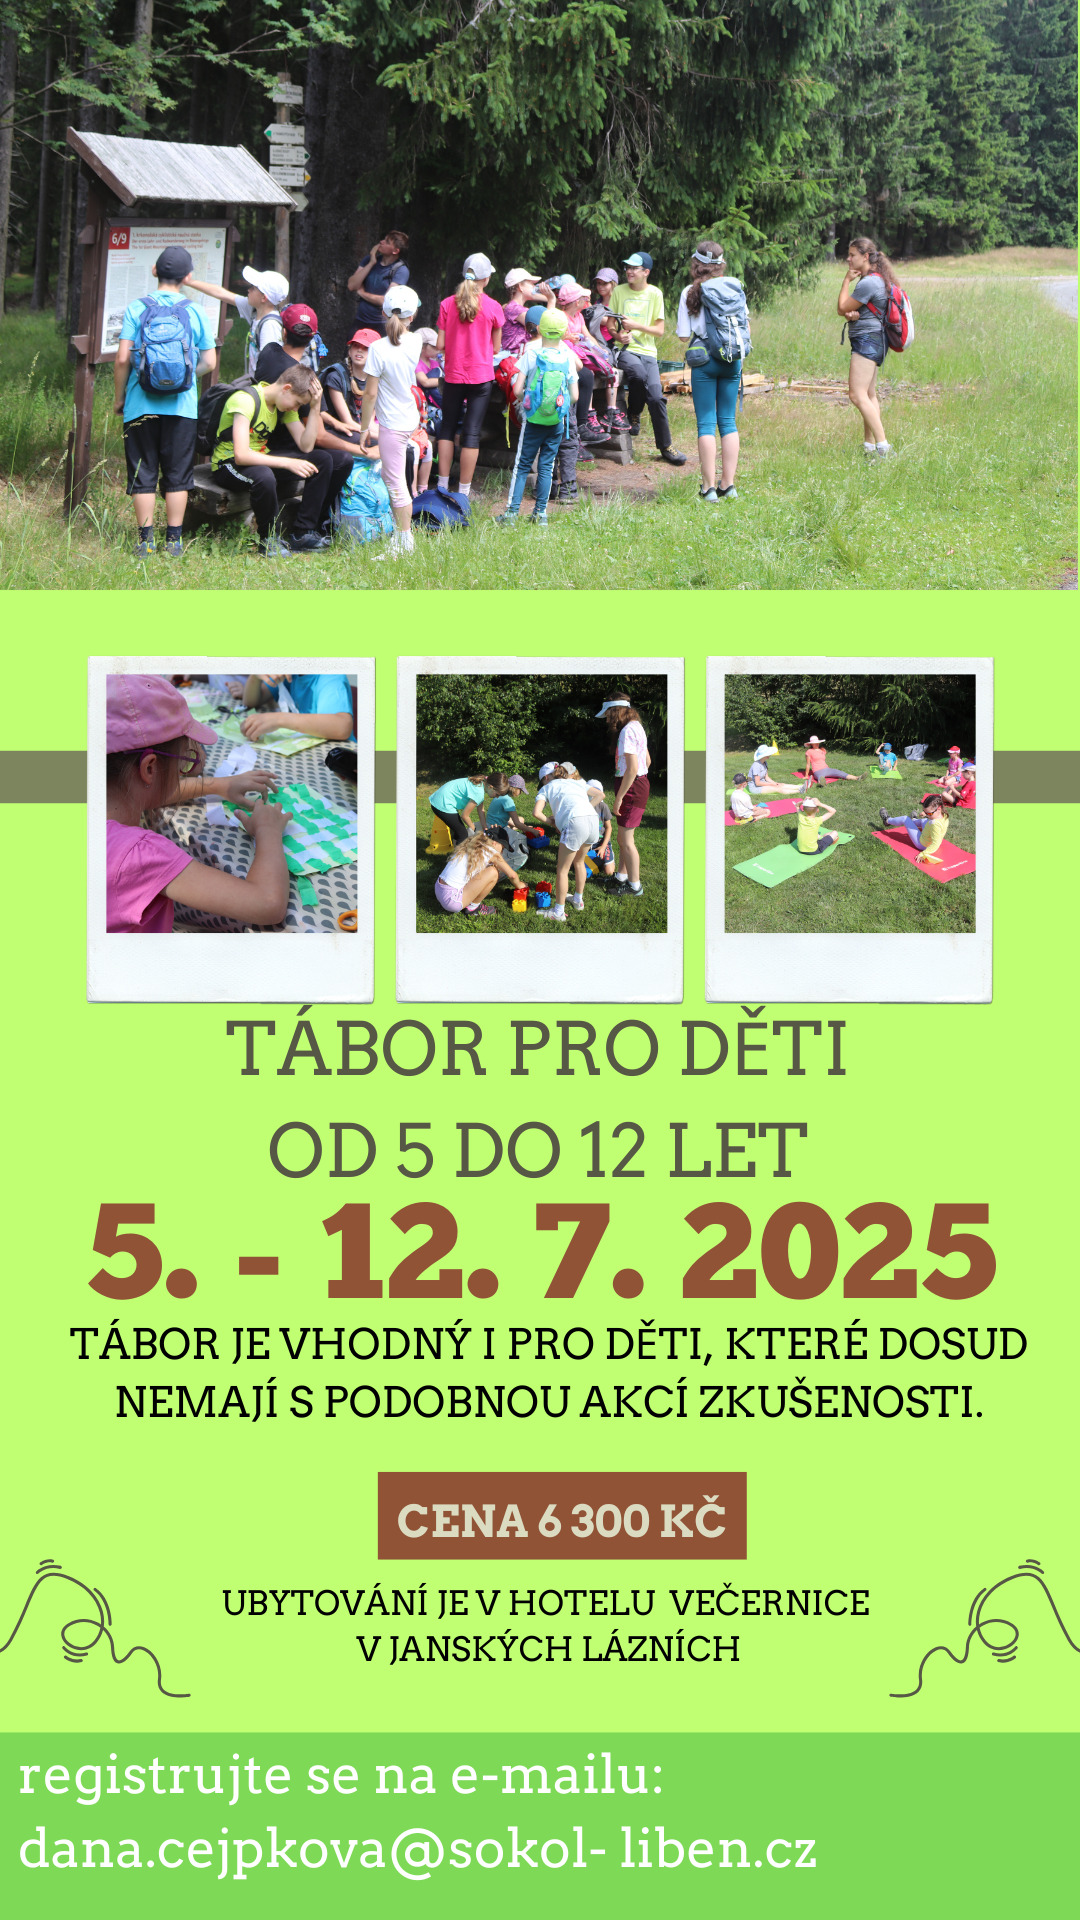
\includegraphics[height=21cm]{./letak_tabor_2025.jpg}
\end{center}
\restoregeometry

\clearpage
\pagestyle{standard}

\post{Co vlastně dělá vzdělavatel?}

\begin{center}
  \textit{Seznámení s~mými předchůdci a proměny vzdělavatelské činnosti.}
\end{center}
Když jsem začala pracovat na tablu s~fotkami cvičitelstva a členstva výboru, nevěděla jsem, do čeho se pouštím. V~archivu je dokladů z~devadesátých let málo a členy výboru jsem určitě nenašla všechny; ale pátrání po nich byla zajímavá exkurze do života naší jednoty a především do životů mých předchůdců.

První vzdělavatel byl František Kodl. V~době obnovení Sokola mu bylo osmdesát let a během období Meteoru působil jako cvičitel "Staré gardy", oddílu seniorů, a oddílu "Základní a rekreační tělesné výchovy", který byl vlastně přejmenovaný Sokol. Skoro každý zná jeho úhledné psací písmo, které zdobilo nástěnky ještě v~době mého působení. V~archivu je několik krabic pečlivě připravených fotoalb – přeložených čtvrtek A3 se třemi fotkami na každé straně (a především s~napsanými jmény!), která vyráběl snad po každé sokolské akci. Fotoalba potom na pár let převzala cvičitelka žactva Iva Duchačová.

Kronika z~Kodlova období je psaná rukopisem místostarosty Josefa Valenty. Pečlivě popisoval první roky naší jednoty po obnovení, dělení majetku s~Meteorem, první opravy v~sokolovně a znovuustanovení celé ČOS. Josef Valenta je druhý člověk, jehož fotografii nemáme na tablu členstva výboru, a dokonce ani starší cvičitelé si na něj nevzpomínají. Můžeme tedy usuzovat, že to byl "manažer v~pozadí", praktický a věcný bratr, který trávil více času v~kanceláři a na úřadech, kde se bil za sokolskou věc. Sokolovnu jsme i díky němu získali poměrně bez průtahů, když se porovnáme s~jinými jednotami, a dokonce jsme z~archivu Meteoru dostali sokolské dokumenty.

Psaní kroniky po Valentovi převzala Ivana Mrklasová, tehdy byla funkce kronikářky volená valnou hromadou. Vnučka prvního starosty Ládi Mrklase staršího působila jako cvičitelka a ještě dlouho se v~naší jednotě objevovala v~loutkářském souboru VHlavěDrát. Zápis v~kronice skončil doslova v~půlce věty na podzim 2008, s~vloženým zbytkem roku na vytištěném papíře připraveném k~opsání.

Další osobou byl Ferdinand Haralík, o~němž není jiná zmínka kdekoliv kromě toho, že byl archivář, naposledy zvolený valnou hromadou v~roce 2000 –⁠⁠⁠⁠⁠⁠ to jen ukazuje, jak je archiv neviditelný a archivní práce nevděčná –⁠⁠⁠⁠⁠⁠ a po zrušení pozice archiváře vzala na sebe péči o~archiv Věra Decastellová. 

Věra měla celý svůj život spjatý s~naším Sokolem: její rodiče se tu poznali, tatínek byl krátce náčelníkem, dlouho vzdělavatelem, maminka náčelnicí a čestnou cvičitelkou, když odešla do sokolského důchodu po 35 letech vedení hodin. Věra poprvé oblékla úbor ještě v~předškolním věku, prožila druhou světovou válku v~domě naproti divadlu, obnovovala Sokol v~letech 1945, 1968 i 1990. Byla skvělá vypravěčka s~impozantní pamětí, ráda se setkávala s~mládeží a vyprávěla na mnohých přednáškách. Účinkovala v~pořadu České televize Neznámí hrdinové –⁠⁠⁠⁠⁠⁠ doporučuji si její díl najít v~archivu ČT. Vítek a Řek s~ní natočili před několika lety asi deset hodin rozhovorů.
V~archivu měla podle ní perfektní pořádek, podle ostatních příšerný nepořádek, ale přesně věděla, kde je co uložené (bohužel jenom ona sama), a na kterýkoliv předmět jsme se zeptali, tak uměla bez zaváhání odpovědět –⁠⁠⁠⁠⁠⁠ co to je, z~jaké doby, kdo je na fotce vyfocený, kde ti lidé žili, čím se živili, kdo tuhle věc Sokolu daroval. Na slavnost výročí položení základního kamene zorganizovala jednotku krojovaných cvičitelů a od té doby se chodilo v~krojích na různé slavnosti; tak jsem se vlastně poprvé dostala za hranice všedních dnů cvičení i já, ještě jako dorostenka.

A~poslední osoba, i když poslední jen časově –⁠⁠⁠⁠⁠⁠ jak se říká anglicky "last, but not least" –⁠⁠⁠⁠⁠⁠ byla Věra Šťastná. Po Františku Kodlovi převzala vzdělavatelskou štafetu i oblíbené seniorské vycházky a držela ji téměř 30 let, od roku 1998, kdy zemřel Kodl, až do své rezignace v~roce 2016. Věru jsem poznala na už dříve vzpomínané slavnosti základního kamene na podzim 2009 a dala se s~ní do řeči až později, když jsem jí pomáhala při spravování fondu sokolských krojů, později jsme spolu připravovaly výstavy, a když pokládala funkci (v~devadesáti letech! a pořád jí to skvěle myslelo), učinila tak s~vědomím, že to "bez ní nespadne". Nebyla tak rázná a výrazná jako Věra Decastellová, a na rozdíl od ní nerada vzpomínala na události války; ale vyprávěla stejně zajímavě a uměla ve svých výstavách jako pohádku vykreslit celý sokolský příběh naší jednoty. 

No a nyní "vedu vzdělavatelák" já, po tom, co jsem od podzimu 2009 sekundovala Věrám. Přišla jsem do Sokola až ve čtrnácti a kromě ikonického dua "Věra \& Věra" (a sestry stály za každou minutu času, kterou si na ně člověk udělal!) nepoznala nikoho ze zmíněných. Na rozdíl od předchůdců nejsem v~důchodovém věku a nemám tolik času. Proto je potřeba dělat věci jinak – jinak neznamená snad hůře ani za každou cenu překonávat předchozí; jen prostě jinak. Už nemáme voleného archiváře, kronikáře ani tiskového mluvčího (poslední byl Čedok – Martin Chlumský). Je jen jedna vzdělavatelka a nezbytný tým pomocníků, kde každý udělá trochu a všichni dohromady udělají moc. 

Mnoho věcí se neděje bohužel vůbec – například na fotoalba jsem narazila až letos a mrzí mě, že se v~nich už nepokračovalo. Kroniku za letošek převzala dorostenka Bára Jeníková, ale chybějí úplně či částečně roky 2009–2023. Nástěnky několik let připravoval Martin Kubů; nevěřili byste, kolik času zabere každý měsíc připravit nové zajímavé povídání, obrázky, výročí a pozvánky na akce do okolních jednot. Martin také spoluorganizoval vycházky do muzeí, o~které po covidu už nebyl takový zájem.

Jsem ráda, že vycházky za kulturou převzali Doupalovi a naši sokolskou kulturu divadelníci v~čele s~principálem Tomášem Troupem, tančírny na sebe vzala Jana Dubská, a tohle všechno dobře šlape v~pravidelném rytmu, krojovaní cvičitelé se střídají na pietních aktech a dalších akcích, čímž zviditelňují Sokol navenek.
Archiv jsme před stěhováním do nových prostor přes rok nahrubo třídili a balili do archivních krabic s~Příborem – Honzou Přibylem a jeho manželkou Aničkou, která pečlivě prošla hudební fond. Sokolské hroby na Korábě udržují mladí cvičitelé sourozenci Květa a Honza Kerhartovi. Velkou akcí bylo zřízení krojovny, kdy každý kus kroje dostal své místo na věšáku, protiprachový obal a cedulku s~evidenčním číslem, a při stěhování se do archivářských ukládacích beden zabalily i dokumenty – zde patří dík starostům Alešovi a Jirkanovi, kteří na ochranný materiál vždy našli peníze v~rozpočtu. Před sletem jsme došívaly dětské kroje (Dáša Francková a Mráťa – Martina Škochová), díky čemuž měla Libeň v~průvodu největší skupinu krojovaných ze všech zúčastněných jednot! A~mnozí další pomohli mnohokrát s~jednorázovými úkoly jako žehlení krojů, sestavení praporů, výroba cvičitelského tabla nebo příprava výstavy. Už jen to nanošení stolů ve třech trvá třetinu času co v~jednom.

Děkuji zde veřejně všem zúčastněným a zároveň tak trochu házím rukavici: Nechcete se někdo z~členů zapsat do historie naší jednoty a vzít si na starost některou z~činností, které aktuálně probíhají nedostatečně nebo vůbec? To jest:
\begin{itemize}
  \item fotoalba (vybrat z~úložiště fotek z~akcí pár kusů za každou, nalepit je na papír a popsat)
  \item nástěnky (1x měsíčně připravit informace o~výročích a pozvánky na akce) 
  \item chybějící zápisy v~kronice (projít minulé Zprávy žactva a zápisy výboru, sepsat nanečisto text ve Wordu a krasopisně opsat do kroniky)
  \item další vycházky za kulturou (2-4x ročně zorganizovat hromadnou návštěvu muzea – toto by měl být dospělý cvičitel)
\end{itemize}

Zakončím slovy bývalého starosty Aleše Müllera, kterými mě tehdy v~srpnu 2018 přesvědčil, abych funkci vzdělavatelky začala dělat oficiálně, když už to stejně tak nějak pár let dělám: "Když to budeš dělat Ty na svých deset procent, je to stále o~sto procent víc, než když to nebude dělat nikdo." A~já k~tomu dodávám: "Když dá deset lidí deset procent každý, dohromady to je sto a ještě víc!"

\signature{Anka Holanová}{vzdělavatelka}

\vspace*{24pt}

\post{Sokolská kapka krve}
Projekt Sokolská kapka krve končí svůj jubilejní 10. ročník. 

Darování krve je celospolečensky navýsost záslužná činnost, kterou se Sokol rozhodl dlouhodobě podporovat. Cílem projektu Sokolská kapka krve je především rozšířit povědomí mezi sokolskou i nesokolskou veřejností o~nutnosti krev darovat a získat nové a hlavně pravidelné dárce. 

Sokolská kapka krve je projekt Zdravotní komise a Předsednictva ČOS. V~rámci tohoto projektu sokolské jednoty hlásí počty dárců krve a počty odběrů za jednotlivá pololetí; na konci roku se výsledky sečtou a zveřejní. Každý dárce pak obdrží odznak a přední jednoty pak věcné odměny. 

První ročník proběhl v~roce 2015 a od té doby počet dárců i odběrů vytrvale stoupá.  Naše jednota se akce účastní od počátku a i u~nás je patrný zvyšující se počet dárců i odběrů. 

Pro představu: v~roce 2023 v~Sokole Libeň krev darovalo 9 členů, kteří absolvovali 23 odběrů, a naše jednota se umístila na 12. místě. Celkově se v~roce 2023 projektu Sokolská kapka krve zúčastnilo 61 jednot a v~nich 354 dárců absolvovalo 930 odběrů. Vítězem se pak stal, jako od začátku vždy, Sokol Komárov, kde 38 dárců absolvovalo 121 odběrů. Od počátku projektu tak Sokolové darovali přes 2500 litrů krve.

Od počátku projektu krev v~Sokole Libeň darovali: 
Z.~Burianová, M.~Burian, N.~Čeněk, J.~Dobis, F.~Dostál, H.~Doupalová, T.~Dragoun, M.~Frost, H.~Hofmannová, V.~Jakoubek, L.~Křemen, M.~Kubů, J.~Kubišta, B.~Novotná, O.~Pokorný, M.~Přibyl, J.~Přech, A.~Přechová, J.~Šmídová, R.~Zdvořilý a L.~Zubáková.

Krevní převody jsou ve zdravotnictví potřeba stále a nikdo dosud nevymyslel, jak krev nahradit. Denně jsou darovanou krví zachraňovány lidské životy, ať již jsou to vážně zranění, matky po těžkých porodech či nemocní leukémií. 

Věřím, že projekt potrvá i nadále a pomůže získat nové a pravidelné dárce.

Veškeré informace o~projektu najdete na nástěnkách v~sokolovně a na www.sokolskakapkakrve.cz. Všechny dotazy též rád zodpovím na e-mailu vit.jakoubek@sokol-liben.cz.

Nezapomeňte mi nahlásit počet odběrů za 2. pololetí (případně i za 1. pololetí, pokud jste zapomněli) do 31. 1. 2025.


\signature{Vít Jakoubek}{zdravotník jednoty a koordinátor projektu}
\vspace*{24pt}

\post{Se Sokolem do divadla}
Směle mohu konstatovat, že kulturní sezóna je v~plném proudu! A~to přesto, že jsme od zahájení školního roku neposlali jedinou pozvánku. Ptáte se, jak je to možné? V~říjnu a listopadu se totiž odehrála již 3 představení, na něž jsme s~ohledem na jejich vytíženost zasílali pozvánky ve velkém předstihu již v~minulém školním roce\,\ldots{}

Naši pomyslnou kulturní sezónu 2024/2025 jsme zahájili 11. října 2024 loutkovým představením o~tom, jak "Hurvínek prodává nevěstu" (63 osob), a nedlouho poté jsme 4. listopadu 2024 zavítali do Rudolfina na vzdělávací program pod názvem "Dvořákova Anglická z~Vysoké" (11 posluchačů).
Prozatím největším "majstrštykem" zůstává naše libeňská návštěva Žižkovského divadla Járy Cimrmana, kde jsme v~rámci oslav 140. výročí založení naší jednoty shlédli představení České nebe. Sešlo se celkem 238 nadšených diváků! Podrobnější popis události najdete v~článku "Oslavy 140 let Sokola Libeň".

Již brzy 12. prosince 2024 vyrazíme do Rudolfina na druhý komentovaný koncert z~cyklu "Kroky do nového světa" – tentokrát se tvůrci inspirovali A. Vivaldim a A. Piazzollou a jsem zvědavý, co si pro nás průvodce pořadem Petr Kadlec a dirigent Marko Ivanovič připravili tentokrát. Jak asi vyzní srovnání Čtvera ročních dob z~Itálie 18. století s~razantním argentinským tangem z~60. let minulého století? On si s~tím však houslista Josef Špaček určitě nějak poradí\,\ldots{}
Pokud by Vás uvedený cyklus zaujal, 20. března 2025 se chystáme na Obrázky z~výstavy s~hudbou M. P. Musorgského. V~rámci možností se mohu pokusit zajistit lístky pro opozdilce.

Věřím, že brzy Vás budu moci pozvat i na nějaké představení "k rychlé spotřebě"\ldots{} A~pokud byste měl někdo zajímavý tip, klidně jej nasdílejte na níže uvedený e-mail.

S~přáním krásného adventu a klidných Vánoc v~kruhu rodinném či sokolském přeje

\signature{Miloslav Doupal}{e-mail: mila.doupal@sokol-liben.cz}
\vspace*{24pt}



% zadní obálka
\clearpage

\pagestyle{blank}
\newgeometry{margin=1cm}

\vspace*{96pt}

\pagecolor{sokolred}
\color{white}

\noindent {\fontsize{48pt}{56pt}\tyrs
se sokolským

\vspace*{24pt}

\noindent nazdar!}

\vspace*{\fill}

% \color{black}
\begin{center}
Vydává Tělocvičná jednota Sokol Libeň, Zenklova 37, Praha 8

\vspace*{12pt}

Na přípravě tohoto čísla se spolu s~autory jednotlivých textů podíleli:

grafická úprava – Martin Burian | jazyková úprava – Martina Waclawičová \\ editoři textů – Vít Jakoubek, Jan Přech
\end{center}

\end{document}